\documentclass[a4paper]{article}

\usepackage{microtype}
\usepackage{fullpage}
\usepackage{mathtools}
\usepackage{amsfonts}
\usepackage{tikz}
\usepackage{pgfplots}
\usepackage{pgfplotstable}
\usepackage{hyperref}
\usepackage[noabbrev,nameinlink]{cleveref}
\usepackage{amsthm}
\usepackage{xcolor}
\usepackage{caption}
\usepackage{subcaption}
\usepackage{setspace}
\usepackage[backend=biber,style=authoryear,maxbibnames=99,hyperref=true]{biblatex} 

\setstretch{1.15}

\addbibresource{src/paper/references.bib}

\usepgfplotslibrary{fillbetween}
\usetikzlibrary{shapes}
\usetikzlibrary{intersections}
\usetikzlibrary{positioning}
\usetikzlibrary{fit}
\usetikzlibrary{arrows}
\pgfplotsset{compat=1.17}

\newtheorem{definition}{Definition}
\newtheorem{observation}{Observation}
\newtheorem{proposition}{Proposition}
\newtheorem{theorem}{Theorem}
\newtheorem{corollary}{Corollary}
\newtheorem{lemma}{Lemma}
\newtheorem{assumption}{Assumption}

\crefname{assumption}{assumption}{assumptions}
\Crefname{assumption}{Assumption}{Assumptions}
\crefname{observation}{observation}{observations}
\Crefname{observation}{Observation}{Observations}

\newcommand{\dt}{\mathrm{d}t}
\newcommand{\ds}{\mathrm{d}s}
\newcommand{\di}{\mathrm{d}i}
\newcommand{\E}{\mathbb{E}}

\newcommand*{\thisdraft}{\normalsize{This draft: \today}} 
\newcommand*{\firstdraft}{\normalsize{First draft: 27 March 2023}} 
\newcommand*{\latestversion}{\normalsize{Latest version: \href{https://stanmart.github.io/ValueOfIntermediation/application.pdf}{stanmart.github.io/ValueOfIntermediation/application.pdf}}}

\definecolor{myblue}{rgb}{0.3, 0.45, 0.69}
\definecolor{myred}{rgb}{0.87, 0.52, 0.32}
\definecolor{mygreen}{rgb}{0.34, 0.68, 0.45}

\pgfplotstableread[col sep=comma]{out/figures/equilibrium_profit_onesided_scale-1_lambda-1.csv}\equilibrium
\pgfplotstableread[col sep=comma]{out/figures/equilibrium_welfare_onesided_scale-0.6_lambda-1.csv}\equilibriumFullSurplusOneSided
\pgfplotstableread[col sep=comma]{out/figures/equilibrium_welfare_twosided_scale-0.6_lambda-1.csv}\equilibriumFullSurplusTwoSided
\pgfplotstableread[col sep=comma]{out/figures/equilibrium_profit_onesided_scale-1_lambda-2.csv}\equilibriumProfitOneSidedHighLambda

\title{Hybrid platforms and bargaining power}
\author{Martin Stancsics \\ \normalsize{University of Zurich}}
\date{\thisdraft \\ \firstdraft \\ \latestversion}

\begin{document}

\maketitle

\begin{abstract}
    This paper explores the effects of a platform selling their own products in addition to acting as intermediaries (hybrid platform) in a setting when bargaining takes place between the platform and the potential entrants.
    It highlights a so-far underappreciated aspect of hybrid platforms: having their own products increases their bargaining power over the other sellers.
    This change in bargaining might lead to lower entry, and thus reduced product variety which in turn can have negative welfare consequences for the consumers.
    The results and methods described in this paper are also applicable to other similar settings, such as vertical integration with a monopolistic upstream supplier.
\end{abstract}


\section{Motivation}

Although market structures resembling various aspects of what we call platforms have existed for some time, the term has only gained widespread usage in the 2000s, with the advent of digitization, and a number of behemoth technology companies playing matchmakers on the internet.
Since then, platforms have become a buzzword in the business world, the subject of increasing regulatory scrutiny, and also a topic of intense academic interest.
Platforms have a number of unique features that make them different from more traditional market structures.
The most prominent of those are multi-sidedness and network effects, which most of the early literature \parencite[for an overview, see][]{rochet2006two} and policy debate \parencite[e.g.][]{fletcher2021consumer,calvano2021market} has focused on.
However, in the more recent years, another important and potentially concerning aspect has been getting more attention: the hybrid operation of certain platforms.
Essentially, this means that platforms act as an intermediary (deciding the rules) and a market participant (competing with other entrants) at the same time.

While hybrid platforms are not a completely new phenomenon, they are becoming more and more common in various industries.
Perhaps the most prominent example is Amazon, which, on the one hand sells its own products, and at the same time hosts ax large number of third-party sellers.
However, examples abound in other industries, as well.
For example, each of the largest digital distribution platforms for computer and smartphone applications (Google Play, Apple App Store and Microsoft Store) sell their own applications besides their third party offerings.
In the video game industry, platform owners studios and publishing games under their own brand is the standard.
Many video streaming services (e.g. Netflix, Amazon Prime Video, Hulu) offer a mix of their own and licensed content.
One can also find examples of similar behavior outside the platform setting, too.
For example, a number of car manufacturers are planning to sell directly to consumers in addition to selling through their dealership networks.

As deciding the rules of the game and competing in it at the same time gives rise to some obvious concerns, policymakers have been paying increasingly close attention to these platforms in the recent years.
Various pieces of legislation have been proposed to regulate, or even ban e-commerce platforms from selling their own products \parencite[][]{phartiyal_2019,reynolds_2022,eu-2022}.
Furthermore, one of the most prominent recent antitrust cases, Microsoft acquiring the video game publisher Activision/Blizzard for a sum of 69 billion USD, is also a case of a platform becoming increasingly hybrid.
This merger not only increased market concentration on the software side of the video game industry, but might also have further implications for the competition between Microsoft as a platform owner and the other game developers.
The deal was under investigation by multiple antitrust authorities, including the US Federal Trade Commission, the European Commission, and the UK Competition and Markets Authority \parencite{livni_merced_2023}.

In parallel to the increasing regulatory interest, the academic literature on the topic of hybrid platforms has also been steadily growing.
\textcite{hagiu2022should} investigate how practices, such as self-preferencing and steering can distort competition on hybrid platforms.
They argue that -- while such practices are problematic and can have negative welfare effects -- with proper regulation the platform selling its own products can be beneficial for consumers.
In contrast to this positive result, \textcite[]{anderson2021hybrid} find that even in the absence of such behavior, allowing hybrid operation might have negative consequences due to platforms having an incentive to exclude competitors from the market.
\textcite[]{gutierrez2021welfare} shows that general conclusions are hard to draw, and welfare effects are platform and product specific.
For example, using a mechanism design approach, \textcite{kang2022contracting} demonstrate that welfare consequences greatly depend on whether the platform faces competition in the upstream market.

This paper aims to contribute to this discussion by examining an important, but so far underexplored aspect of platforms: the bargaining power disparity between them and the other market participants, and how this disparity is affected by the platforms' hybrid operation.
I propose an analytically tractable model of a which captures many important aspects of bargaining between one large and a continuum of small players: namely a hybrid platform facing a continuum of potential entrants.
I show that, in the presence of bargaining, hybrid operation can indeed have negative welfare consequences for consumers.
This result is particularly striking in this otherwise distortion-free\footnote{
    In the benchmark model without bargaining, the platform's hybrid operation does not affect consumer welfare.
} setting. 
The intuition is that hybrid operation increases the platform's bargaining power against the entrant sellers.
This in turn leads to a higher entry fee, fewer entrants, then results in lower consumer surplus.
These observations constitute a so-far overlooked aspect of hybrid platforms that policymakers should be aware of.
Due to the relative generality of this model, these results are applicable not only to hybrid platform, but to other similar settings, such as upstream producers having their own downstream outlets, or retailers with private labels, as well.

Many of the results are not tied to the specifics of the model, but are more general instead.
They do not depend on a specific demand structure and investment cost assumptions, and there is even some flexibility to the assumptions about bargaining outcomes.
I show that, even in such stylized setting, some interesting observations can be made about the effects of hybrid operation. 
In particular, when the platform's and the potential entrants' products are substitutes, increasing the platform's product variety will lead to a decrease in the number of entrants.
I also give sufficient conditions for this decrease in entry being so large as to cause a decrease in total profits, as well.

The closest model to the one proposed in this paper is \textcite{anderson2021hybrid}.
The key difference between the two boils down to how the entry fee is decided.
In \textcite{anderson2021hybrid}, the platform sets a percentage entry fee, and the entrants decide whether to enter or not.
In contrast to this, I assume that (1) platforms charge a lump-sum entry fee and that (2) this entry fee is the result of a negotiation process\footnote{
    The bargaining process is modeled using a solution concept from cooperative game theory, namely the Shapley-value.
    This allows for a tractable analysis while at the same time capturing many of the important features of bargaining.
    Examples of this approach in the industrial organization literature include \textcite{montez2007downstream}, as well as \textcite{hart1990property}, \textcite{levy1997individual}, \textcite{inderst2003bargaining} and \textcite{brugemann2019intra} among others.
}
between the platform and the entrants.
The second point is a novelty not only compared to \textcite{anderson2021hybrid}, but also to the existing literature on hybrid platforms.
Furthermore, in contrast to \textcite{hagiu2022should}, this model is free from any distortive behavior, such as self-preferencing or steering, and the negative results are purely driven by changes in the platform's bargaining position.

The set of more general results in this paper go beyond the aforementioned studies in the sense that they illuminate the effects of hybridness as a more abstract phenomenon, and thus also highlight the similarities between the hybrid platform literature and adjacent ones.
Certain structures, such as vertical relationships, or even traditional retail stores share a number of features with platforms (notably, the presence of a dominant, indispensable entity), and can be modeled in much the same way.
Therefore, the methodology and results in this paper are also of interest to researchers studying questions such as retailers having their own private labels \parencite{steiner2004nature} or vertical integration in upstream-downstream markets \parencite{hart1990vertical,aghion2006vertical}.
\textcite{de2005vertical} and \textcite{montez2007downstream}, in which bargaining between the upstream and downstream firms take the center stage, are particularly closely related.
Among empirical studies in related settings, \textcite{ho2017insurer} looks at the effect of insurer competition on health care prices, while \textcite{crawford2018welfare} explores the effects of vertical integration on television markets.

This paper is also related to various other strands of the industrial organization literature.
Most generally, it is a contribution to the research agenda on understanding platforms and their role in the economy \parencite[e.g.][]{rochet2003platform,hagiu2004optimal,armstrong2006competition,evans2011platform,lee2014competing}.
Furthermore, it is somewhat adjacent to the literature on the importance of exclusive content \parencite[e.g.][]{hagiu2011exclusivity,lee2013vertical,dou2014sell,weeds2016tv}, with the difference that instead of exclusive content giving an advantage against competing platforms, in this paper, own products provide an advantage over potential entrants.
More generally, many results and concepts of this paper are also applicable outside the context of (multi-sided) platforms.

Finally, this paper also belongs to the not too large set of models using concepts from cooperative game theory in an industrial organization setting.
Such examples include the aforementioned \textcite{montez2007downstream}, as well as \textcite{hart1990property}, \textcite{levy1997individual}, \textcite{inderst2003bargaining} and \textcite{brugemann2019intra}, among others.
In contrast to the majority of those, which focus on games with a finite number of players, I utilize an oceanic game (a continuum of small players instead of a finite number), and demonstrate that this can considerably simplify the analysis in certain cases.
Therefore, the modeling approach presented in this paper may be of use in other settings as well.

The rest of the paper is organized as follows.
In \cref{sec:model}, I introduce two model of hybrid platforms: a benchmark with the platform setting an entry fee unilaterally, and the main model, where the platform and the fringe firms engage in bargaining.
After that, \cref{sec:results}\footnote{
    \Cref{sec:more_general} explores the generalizability of these results, and highlights some common themes in settings with hybrid behavior.
} demonstrates that the two have very different implications for consumer welfare.
\Cref{sec:extensions} then examines the effect of different assumptions about the bargaining process.
Finally, \cref{sec:conclusion} summarizes the results and discusses possible future work.


\section{Model}
\label{sec:model}

This section introduces the model used throughout the paper.
% TODO: better motivation
I use the terms ``platform'' and ``fringe sellers'', and present my ideas in the context of an intermediated market, such as an online marketplace or an application store.
However, the model is quite general, and the results apply to a broader class of settings, such as vertical markets where the upstream firm can sell directly to consumers, or retail stores with their own private labels.

Assume that there are two types of players in the market: a platform $P$, a continuum of fringe sellers $F_i$ ($i \in [0, N_F$]) and a continuum of consumers $C_j$ ($j \in [0, 1]$).
The fringe firms have one product each, which they can only sell through the platform.
Without the platform, they make zero profits.
In addition to acting as an intermediary between the fringe and the consumers, the platform itself may also produce and sell a number of products directly to the consumers.
If it does, it is referred to as a hybrid platform.

The main distinguishing feature of this model is that, instead of assuming that entry fees or royalties are set by the platform and the fringe treat it as take it or leave it offers, I assume that the platform and the fringe engage in some kind of bargaining over their total profits.
The bargaining rule, as well as other details of the model, are described in the rest of this section.


\subsection{Overview}

There is an infinite measure of fringe firms, who are deciding whether to enter the market.
Entering has two, separate costs: an exogenous investment cost $I_F$, and the lump-sum platform entry fee $K_F$.
One can conceptualize the first as usual fixed costs, such as the cost of setting up production, or designing a product.
Meanwhile, the second is a payment to the platform for using its services.
While percentage fees are more common both in the literature and in practice, I assume a lump-sum fee for a few reasons.
First, and most importantly, revenue-based fees enter the entrants' pricing decision, and thus create a channel through which platforms distort competition.
I want to show that even in the absence such distortions, hybrid platforms can have a significant impact on competition.
Furthermore, due to this distortion, the resulting game could not be represented as a transferable utility game, and the proposed solution concept would not be applicable.
Finally, lump-sum fees do make sense in settings when individual negotiation takes place and contracts are not standardized.

In the benchmark model, the game starts by the platform announcing and committing to an entry fee $K_F$.\footnote{
    With no commitment power, but the ability to set any prices after fringe firms make their investment decisions, the platform would charge an entry fee that would make the fringe profits zero \emph{sans the investment cost}.
    This would lead to a trivial equilibrium, where no firm enters.
}
In the bargaining case, the platform cannot commit to entry fees at this point.
Next, each fringe firm decides whether to create a product at cost $I_F$ and enter the market.
In the bargaining model, the entry fee is decided at this point as a result of some negotiation\footnote{
    The negotiation process, or rather its outcome is described in detail in \cref{sec:cooperative_game}.
} between the platform and the firms that have made the investment.
After this, the firms that made the investment pay the platform entry fees, too.

From this point on, the game proceeds in the same way in both models.
The platform and the fringe firms simultaneously choose the prices for their products, engaging in monopolistic competition.
Finally, consumers make their purchase decisions, and profits are realized.

In the model with bargaining, the platform and the fringe distribute total profits according to their Shapley values.
One can also think of the latter as agreeing on an entry fee that makes final profits net entry fees equal to the Shapley value of the various players.

The main difference between the benchmark and the bargaining model is in determining the entry fee $K_F$.
In the former, the platform unilaterally sets the fee, and the fringe treats it as a take it or leave it offer.
On the other hand, in the bargaining model, I assume that the entry fee is the result of a negotiation between the parties.
\Cref{fig:timing} illustrates this difference.

\begin{figure}
    \centering
    \begin{subfigure}{0.45\textwidth}
        \centering
        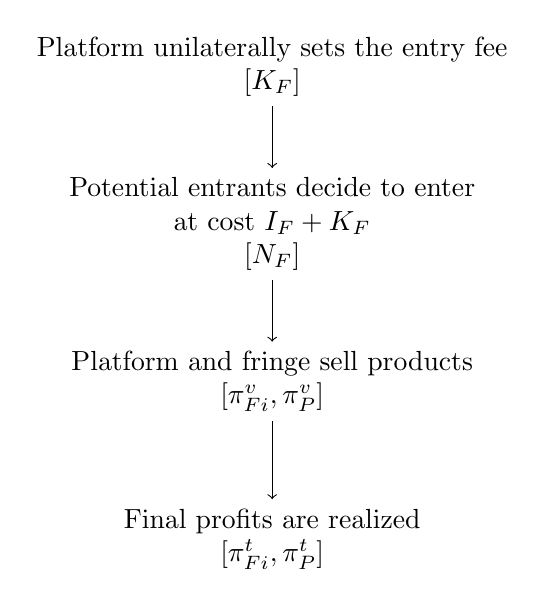
\begin{tikzpicture}[node distance=2cm, auto]
            \node[align=center] (entry_fee) {Platform unilaterally sets the entry fee \\ $[K_F]$};
            \node[align=center] (entry_decision) [below of=entry_fee] {Potential entrants decide to enter \\ at cost $I_F + K_F$ \\ $[N_F]$};
            \node[align=center] (sales) [below of=entry_decision] {Platform and fringe sell products \\ $[\pi_{Fi}^v, \pi_P^v]$};
            \node[align=center] (final) [below of=sales] {Final profits are realized \\ $[\pi_{Fi}^t, \pi_P^t]$};
            \draw[->] (entry_fee) -- (entry_decision);
            \draw[->] (entry_decision) -- (sales);
            \draw[->] (sales) -- (final);
        \end{tikzpicture}
        \caption{Benchmark model (platform sets the entry fee unilaterally)}
    \end{subfigure}
    \hfill
    \begin{subfigure}{0.45\textwidth}
        \centering
        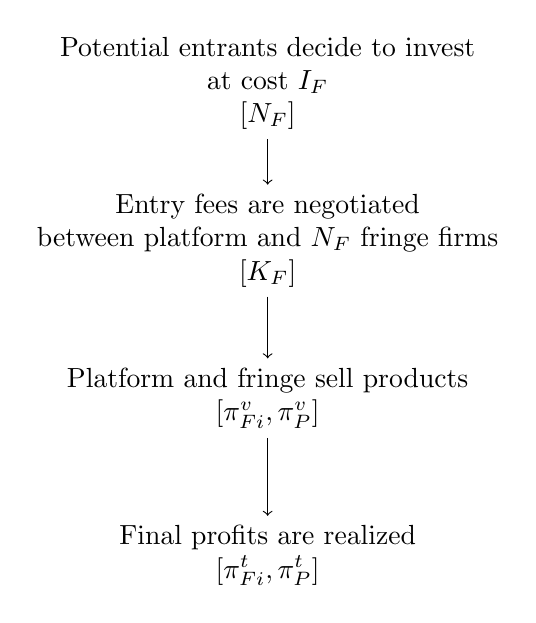
\begin{tikzpicture}[node distance=2cm, auto]
            \node[align=center] (entry_decision) {Potential entrants decide to invest \\ at cost $I_F$ \\ $[N_F]$};
            \node[align=center] (entry_fee) [below of=entry_decision] {Entry fees are negotiated \\ between platform and $N_F$ fringe firms \\ $[K_F]$};
            \node[align=center] (sales) [below of=entry_fee] {Platform and fringe sell products \\ $[\pi_{Fi}^v, \pi_P^v]$};
            \node[align=center] (final) [below of=sales] {Final profits are realized \\ $[\pi_{Fi}^t, \pi_P^t]$};
            \draw[->] (entry_decision) -- (entry_fee);
            \draw[->] (entry_fee) -- (sales);
            \draw[->] (sales) -- (final);
        \end{tikzpicture}
        \caption{Bargaining model (platform and fringe negotiate over the entry fee)}
    \end{subfigure}
    \caption{Timing of the models}
    \label{fig:timing}
\end{figure}

In the rest of this section, I describe each step in detail, starting from the end of the game and working my way back to the beginning.

\subsection{Demand}
\label{sec:demand}

Imagine that there is a unit mass of consumers, looking to buy one product each.
They choose from a continuum of products, which are either produced by the fringe (indexed by $F_i$), by the platform ($P_i$) and a unit mass of outside options ($0_i$).
Customer $j$ derives the following utility from buying product $T_i$:
\begin{align*}
    u_{T_i}^j = v_{T_i} - p_{T_i} + \mu\epsilon_{T_i}^j \quad \text{for } T_i \in \{F, P\},
\end{align*}
where $v_{T_i}$ is the value of product $T_i$, $p_{T_i}$ is its price, and $\epsilon_{T_i}^j$ is an idiosyncratic taste shock.
Throughout this section I assume that the value of each product within its category is the same.
I.e., $v_{T_i} = v_T \, \forall\,i$.
This is to simplify the analysis, but is not crucial for the results.

$\epsilon_{T_i}^j$ is assumed to be independent and identically distributed (i.i.d.) across consumers and products, and follow a standardized Type I Extreme Value distribution.
This distributional assumption, along with the fact that each consumer consumes only one product, will lead to a tractable, logit-form demand function.

\subsubsection{Production}

Each (horizontally differentiated) product is produced by a single, monopolistically competitive (fringe) seller.
The production entails a constant marginal cost $c_{T_i}$.
As with the value, I assume that the marginal cost is the same for all products: $c_{T_i} = c_T$.
Facing the demand described in the previous paragraphs, the sellers choose their price $p_{T_i}$ to maximize profits.
The price of the outside option is normalized to zero.

The pricing decision of the fringe sellers is rather straightforward, due to their infinitesimal market share: they do not have to take into account the effect of their prices on the aggregate demand.
This normally is not the case for the platform, as it can affect a non-zero measure of the prices.
Therefore, when setting the price for product $P_i$, it would optimally like to take into account how it affects demand on its other products $P_j$ $(j \neq i)$.
Despite this, I assume that the platform prices its products as if they were produced by separate, monopolistically competitive sellers.

I do this for a number of reasons.
For one, it simplifies the analysis without affecting the main results qualitatively.
More importantly, it lets me focus on the main question of this paper: how the platform's hybrid operation affects the bargaining power.
If the platform priced its products strategically, there would be a quite mechanical effect that an increase in the number of products would lead to an increase in optimal prices, which would in fact decrease consumer surplus.
This hard to disentangle the effects of hybrid operation from the effects of strategic pricing.
Therefore, this assumption can be seen as a best-case scenario for consumers, and the results can be interpreted as a lower bound on the negative effects of hybrid operation.
For a more thorough discussion of this assumption, see \cref{sec:separate_pricing}.

Finally, this assumption is not as unrealistic as it might seem at first.
For example, the platform might be producing its products through a number of subsidiaries, which are legally separate entities, thus having no control over operational decisions, but still getting the profits from the sales.
Alternatively, there might be some kind of internal competition between the different product teams, which would lead to a similar outcome.

\subsection{Fringe entry and platform fees}

\subsubsection{Benchmark case}

I assume that there is a continuum of potential fringe entrants, indexed by $i \in \mathbb{R}^+_0$.
Each of them can create a product at an exogenous investment cost $I_F$.
If they decide not to, they make zero profits and do not participate in the later stages of the game.
Furthermore, these firms can only sell their products through the platform, for which the platform can charge a lump-sum entry fee $K_F$.
The timing of these decisions is as follows: (1) the platform sets and commits to an entry fee $K_F$, (2) the fringe firms decide whether to enter the market, and (3) the firms that have entered pay the entry fee to the platform.

\subsubsection{Bargaining case}
\label{sec:model_bargaining}

In contrast to the benchmark model, in this case, the platform cannot commit to an entry fee: it is decided as a result of a negotiation between the platform and the fringe firms.
For this reason, the timing of the model is also different.
First, the fringe firms decide whether to invest in creating a product at cost $I_F$.
After this, the platform and the firms that have made the investment negotiate the entry fee.
Finally, the firms that have entered pay the entry fee to the platform.

In order to keep the model tractable I model the negotiation process in a reduced form manner.
In particular, I assume that the platform and the entrants agree on an entry fee $K_F$, which makes the total profits net entry fees equal to the Shapley value of the players.\footnote{
    One simple extension would be to use the more general concept of random order values \parencite{weber1988probabilistic}.
    \Cref{sec:cooperative_game_weighted} takes a step in this direction by introducing bargaining weights and utilizing the weighted value.
}
This way of modelling bargaining outcomes has many precedents in the industrial organization literature \parencite[e.g.][]{montez2007downstream,hart1990property,levy1997individual,inderst2003bargaining,brugemann2019intra} and has a number of appealing properties.
For example, it is closely related to the marginal contributions of the players to the total value, and, as it will be shown, it is also quite intuitive in terms of comparative statistics.
Furthermore, and perhaps more importantly, there are a number of ways to place it on non-cooperative microfoundations by setting up non-cooperative games for which the Shapley value is a subgame perfect equilibrium \parencite[e.g.][]{gul1989bargaining,hart1996bargaining,stole1996organizational}.\footnote{
    For a possible microfoundation of this specific model, see \cref{sec:bargaining_microfoundation}.
}

For the Shapley value (or any other cooperative solution concept) to be well-defined, the corresponding coalitional game must be specified.
\Cref{sec:cooperative_game} describes it in detail, but in short, the idea is the following: given any subset of the players (coalition), players can predict total, industry-wide profits assuming the monopolistic competition described previously.
This is taken as the value of that coalition, thus defining a characteristic function.
Then, every firm (including the platform) will get their average marginal contribution this industry-wide profit (with the average taken over all possible orderings of the firms).

In practice, it looks like the following.
Assume that $N_F$ fringe firms choose to invest in creating a product in the first stage of the game.
Now, for every $s N_F$ ($s \in [0, 1]$), calculate the total profits that would be realized if the platform and $n_f$ fringe firms were the only players in the market, and they engaged in monopolistic competition as described in the previous paragraph.
Let us denote these profits by $\pi^v_{F}(N_P,s N_F)$ and $\pi^v_{P}(N_P,s N_F)$, and the corresponding industry-wide total profits by $\Pi$ and $\Pi(N_P,s N_F, N_C)$.

\begin{proposition}
    \label{prop:shapley_value}
    The Shapley value of the platform and the fringe firms, and thus final total profits, are given by:
    \begin{align*}
        \pi^t_P(N_P, N_F) &= N_C \int_0^1 \Pi(N_P,s N_F) \ds, \\
        \pi^t_F(N_P, N_F) &= N_C \int_0^1 \partial_2 N_F \Pi(N_P,s N_F) \ds.
    \end{align*}
\end{proposition}


\subsection{Equilibrium}

For both models, the previous sections describe a perfect-information extensive-form game.
As a consequence, the solution concept I use is the subgame perfect equilibrium.
As the platform's product variety ($N_P$) is assumed to be exogenous, the only strategic variables are (1) the fringe players' entry decisions, (2) the platform's entry fee (only in the benchmark model), and (3) the prices of the products.

Furthermore, the game can be solved via straightforward backward induction.
In both models, the final subgame is simply a game of monopolistic competition with horizontally differentiated products.
In the benchmark model, it is preceded by the platform setting the entry fee, while in the bargaining model the entry fee is set according to the previously described rule (which in turn can be motivated by an extensive form game).
Finally, the first stage of the game is the fringe firms' investment decision.
Due to the outside option being normalized to zero, the fringe firms will enter the market if and only if the expected profits from doing so are positive, leading to the usual free entry condition.


\section{Results}
\label{sec:results}

I will now present the main results of the model, again, starting from the final subgame and working backwards.
For each subgame, I also demonstrate that the equilibrium exists and is unique, and therefore the complete game also has a unique equilibrium.

\subsection{Demand and producer profits}
\label{sec:results_demand}

As the final, price-setting subgame is the same in both the benchmark and the bargaining model, the results in this subsection apply to both.
Discrete choice models with type I Extreme Value errors give rise to a logit-type demand function \parencite[e.g.][]{small1981applied}.
More specifically, \textcite[]{anderson2021hybrid} utilize the exact same utility structure as in \cref{sec:model}, and show that it gives rise to the following demand function.
\begin{proposition}
    \label{prop:demand_function}
    The demand for product $i$ of producer $T \in \{P, F\}$ is given by:
    \begin{align*}
        x_{T_i} = \frac{\exp\left( \frac{v_T - p_{T_i}}{\mu} \right)}{A}
    \end{align*}
    where
    \begin{align}
        A = \int_0^{N_F} \exp\left( \frac{v_F - p_{F_i}}{\mu} \right) \di + \int_0^{N_P} \exp\left( \frac{v_P - p_{P_i}}{\mu} \right) \di + 1.
        \label{eq:aggregate}
    \end{align}
\end{proposition}

Let us call $v_T - p_{Ti}$ the net value of product $i$.
As one would expect, demand is increasing in this net value, and decreasing in the competitors' net values.
Furthermore, demand for each product is increasing in $\mu$, which describes the degree of product differentiation or the importance of taste shocks.
Finally, notice that, as each producer is infinitesimal, its pricing decision does not affect the aggregate $A$.
This last property makes the optimal prices and profits of the producers very simple, as shown in the next proposition.
\begin{proposition}
    \label{prop:optimal_profit}
    The profit maximizing price for product $T_i$ is
    \begin{align*}
        p^*_{T_i} = c_T + \mu,
    \end{align*}
    and the profit from selling that product is
    \begin{align}
        \pi^{v*}_{T_i} = \mu \frac{\exp \left( \frac{v_T - c_T - \mu}{\mu} \right)}{A}.
        \label{eq:optimal_profit}
    \end{align}
\end{proposition}

For ease of notation, let us define the following:
\begin{align*}
    V_T = \exp \left( \frac{v_T - c_T - \mu}{\mu} \right).
\end{align*}
$V_T$ can be thought of as the value of the product, also accounting for marginal costs and taste heterogeneity.
In this logit demand system, the value of the product is the only parameter that matters for market shares and profits.
In fact, equilibrium per-product demand and variable profit can simply be expressed as $V_T/ A$ and $\mu V_T/ A$, respectively, where
\begin{align*}
    A = N_P V_P + N_F V_F + 1
\end{align*}
denotes the total aggregate.

Finally, another important feature of this demand system is that, assuming optimal pricing, consumer welfare only depends on the size of the aggregate \parencite{anderson2020aggregative}.
In particular, consumer surplus is proportional to the logarithm of the aggregate: $CS = \mu \log(A)$. This fact makes welfare analysis rather simple in this setting.

\subsection{Benchmark: platform sets entry fee unilaterally}

Let us now examine entry fees and fringe entry decisions in the benchmark model.
Recall that there is an infinity of potential fringe entrants looking to enter the market.
Therefore, total profits in equilibrium must be zero.
Combined with the  profit function, this gives the following expressions for the equilibrium number of fringe firms and the equilibrium size of the aggregate.
\begin{proposition}
    \label{prop:equilibrium_aggregate_benchmark}
    If entry costs $I_F$ and $K_F$ are low enough, the equilibrium size of the aggregate is
    \begin{align}
        A = \mu \frac{V_F}{K_F + I_F}.
        \label{eq:aggregate_eq}
    \end{align}
    and the equilibrium number of fringe firms is
    \begin{align*}
        N_F = \frac{\mu}{K_F + I_F} - N_P \frac{V_P}{V_F} - \frac{1}{V_F}.
    \end{align*}
    Otherwise,  $N_F = 0$ and the equilibrium size of the aggregate is
    \begin{align*}
        A = N_P V_P + 1.
    \end{align*}
\end{proposition}
Note that in the first case (\cref{eq:aggregate_eq}), the size of the aggregate does not depend on the platforms' product variety or the platform's product value.
The intuition behind this is that per-firm fringe profits only depend on these factors indirectly, through the size of the aggregate.
Therefore, the zero profit condition for the fringe firms pins down the aggregate in equilibrium (as long as the fringe is feasible).
That is, an increase in $N_P$ will simply replace some fringe entrants, but the free entry condition will pin down the same aggregate regardless of the number of platform products.

Now let us turn to the optimal entry fee set by the platform, and its total profits (consisting of revenue from its own sales and the collected entry fees).
The following proposition establishes these both for the hybrid and the pure retail regimes, and \cref{fig:entry_fee,fig:platform_profits} demonstrates them graphically.

\begin{theorem}
    \label{prop:optimal_entry_fee}
    The optimal entry fee when the platform is operating in the hybrid regime is unique and given by
    \begin{align*}
        K_F^* = \sqrt{\mu I_F V_F} - I_F.
    \end{align*}
    The platform's total profit in this case is
    \begin{align*}
        \pi_P^{t} = \mu - 2\sqrt{\frac{I_F \mu}{V_F}} + \frac{I_F}{V_F} (N_P V_P + 1).
    \end{align*}
    When the optimal mode of operation is retail, the platform's profit is
    \begin{align*}
        \pi_P^{t} = \pi_P^{v} = \mu \frac{ N_P V_P}{N_P V_P + 1}.
    \end{align*}
\end{theorem}

First, let us look at the case when the platform finds it optimal to operate in the hybrid regime.
Notice that the optimal entry fee does not depend on either the platform's product value or product variety (\cref{fig:entry_fee}).
This is because due to the lump-sum nature of the entry fee, the platform can extract all the surplus from the fringe firms, and thus chooses $K_F$ to maximize total industry profits.
The latter is essentially a function of the aggregate, minus the investment costs of the fringe firms.
As I have shown in \cref{prop:equilibrium_aggregate_benchmark}, the aggregate is independent of the platform's product variety in the hybrid regime, and therefore the optimal entry fee is also independent of it.

On the other hand, the platform's profit is increasing in the number of its products (\cref{fig:platform_profits}).
This is a rather mechanical result: the platform's product variety is exogenous, and therefore possible investment costs are not modeled.
If the platform is operating in the hybrid regime, less fringe firms are needed to achieve the (fixed) equilibrium aggregate, therefore there is less expenditure on (essentially wasted) investment costs.
Consequently, in the hybrid regime, the derivative of optimal profits with respect to the platform's product variety is simply the fringe's investment cost, adjusted for the possible difference in product value.
\begin{corollary}
    \begin{align*}
        N_F > 0 \implies \frac{\partial \pi_P^t}{\partial N_P} = \frac{V_P}{V_F} I_F.
    \end{align*}
\end{corollary}
This results also have implications for what would happen if the platform's product variety was an endogenous choice.
It would only choose to operate in a hybrid mode if it had some advantage over the fringe firm's products (either in investment cost, production cost, or product value).
Otherwise, it would simply operate as a pure intermediary, and the number of fringe firms would adjust to the equilibrium aggregate.

Another important corollary of \cref{prop:optimal_entry_fee} is that consumer welfare is also unaffected by the platform's product variety in the hybrid regime.
\begin{corollary}
    \label{prop:consumer_surplus_benchmark}
    \begin{align*}
        N_F > 0 \implies \frac{\partial CS}{\partial N_P} = 0.
    \end{align*}
\end{corollary}
This result is a direct consequence of the facts that the aggregate is independent of the platform's product variety in the hybrid regime, and that consumer surplus is a monotone increasing function of the aggregate.

Next, let us turn to the case when the platform finds it optimal to operate as a pure retailer.
In this case, the only products on the market are the platform's own products.
Therefore, quite mechanically, the aggregate, and thus consumer surplus, are increasing in the number of the platform's products.
\begin{corollary}
    \begin{align*}
        N_F = 0 \implies \frac{\partial CS}{\partial N_P} = \frac{\mu V_P}{(1 + N_P V_P)^2} > 0.
    \end{align*}
\end{corollary}

Finally, note that the profit of the platform under the hybrid regime is higher than under the retail regime, whenever the former is feasible.
Therefore, for a given $N_P$, the platform prefers to operate in hybrid mode, and does not want to exclude fringe firms from the market.
This fact, together with the previous corollaries, implies that the platform's product variety always has a weakly positive effect on consumer welfare.\footnote{
    This is in contrast to \textcite{anderson2021hybrid}, where a platform operating in hybrid mode sets higher royalties to create a price advantage for its own products.
    The reason for this difference lies in the type of entry fee: they assume a revenue-based, proportional fee, which distorts prices.
    In contrast, in this paper, I assume a non-distortive, lump sum fee.
}
\begin{corollary}
    \begin{align*}
        \frac{\partial CS}{\partial N_P} \geq 0.
    \end{align*}
\end{corollary}
It either has no effect (hybrid operation), or it increases the aggregate (pure retailer), and thus consumer surplus.
\Cref{fig:fringe_entry_eq} illustrates this effect.

Finally, these results also suggest that if the platform's product variety (and thus also the pure marketplace/ hybrid mode decision) was endogenous, an improvement in the platform's product (either higher value or lower cost) would also have a weakly positive effect on consumer welfare.
Therefore, it suggests that platform's having their own products are always weakly beneficial for consumers.
This surprising result depends on a number of -- admittedly unrealistic -- assumptions.
Namely, the lump-sum nature of the entry fee, no entry fee for consumers, and the platform pricing its products as if they were produced by separate sellers.
Therefore, one should not take this result as a conclusion applicable to the real world, but as a best-case benchmark.
On the other hand, these assumptions are also why this model is so useful as a benchmark: as I show in the next subsection, even with these assumptions in place, the platform's product can have a negative effect on consumer welfare if the entry fee is set through bargaining.

\subsection{Bargaining: platform and entrants negotiate over entry fees}

Let us now turn to the main contribution of this paper: the case where the platform and the fringe firms negotiate over the division of profits.
As the platform cannot choose and commit to an entry fee, the first two periods are switched compared to the benchmark model.
The game starts by fringe firms' investment decisions, after which, in the second period, bargaining takes place between the platform and the entrants to determine the entry fee.

As described in \cref{sec:model_bargaining}, the participants negotiate over the aggregate profits that they expect to obtain in the subsequent period (assuming the same non-collusive, monopolistic pricing, as before).
From \cref{eq:optimal_profit}, the total profit achieved by the platform and $N_F$ fringe firms is given by
\begin{align*}
    \Pi(N_P, N_F) = \mu \frac{n V_F + N_P V_P}{n V_F + N_P V_P + 1}.
\end{align*}
Bargaining outcomes are determined according to Shapley values, given by \cref{prop:shapley_value}.
Based on these, one can even obtain closed-form expressions for platform and fringe profit shares for this class of demand systems.
\begin{proposition}
    \label{prop:platform_profits_bargaining}
    The platform's total profits are
    \begin{align*}
        \pi^t_P = \mu \left[ 1 - \frac{\log \left(1 + \frac{N_F V_F}{N_P V_P + 1} \right)}{N_F V_F} \right].
    \end{align*}
    The total profits of the whole fringe (excluding investment costs) are given by
    \begin{align*}
        \pi^t_F = \mu \left[ \frac{\log \left( 1 + \frac{N_F V_F}{N_P V_P + 1} \right)}{N_F V_F} - \frac{1}{N_P V_P + N_F V_F + 1} \right].
    \end{align*}
\end{proposition}

Now let us turn to how the platform's dual mode operation affects product variety and consumer welfare.
I start by showing that the equilibrium is unique in this case, as well.
This, and a few other results in this section\footnote{
    These results do not actually rely on the specific logit demand system.
    As long as the fringe profit function has the property described in \cref{lem:shape_of_fringe_profit}, and the total profit function satisfies some assumptions, the results hold.
    \Cref{sec:more_general_results} provides more detail on the necessary assumptions.
}, rely on the following lemma.
\begin{lemma}
    \label{lem:shape_of_fringe_profit}
    For any $N_P, N_F \geq 0$, the fringe profit function is either concave or decreasing in $N_F$:
    \begin{align*}
        \frac{\pi_F^t(N_P, N_F)}{\partial N_F} < 0 \text{ or } \frac{\partial^2 \pi_F^t(N_P, N_F)}{\partial N_F^2} < 0 \quad \forall\, N_P, N_F \geq 0.
    \end{align*}
\end{lemma}
This lemma states that the fringe profit function is hump-shaped in the sense that it starts with an increasing, concave part, after which it may turn into a decreasing (but not necessarily concave or convex) function of $N_F$.
\Cref{fig:equilibrium} illustrates this property.

While this lemma's main purpose is to help establish the other, more interpretable results in this chapter, it is also interesting in its own right.
It shows that the number of fringe firms have a non-monotonic effect on the total profits of the fringe.
That is, even though industry-wide profits are increasing in $N_F$, the share that the fringe can obtain may decrease after a certain point, not only in relative terms, but also in absolute terms.
The underlying reason is that as the number of fringe firms increases, due to their substitutability with each other, their bargaining power decreases.
This decrease can be large enough to offset the total pie getting larger.

\begin{figure}[ht]
    \centering
    \begin{tikzpicture}[xscale=2,yscale=2,samples=200]
        \draw[->] (0,0) -- (0,2);
        \draw[->] (0,0) -- (5.5,0) node[below] {$N_F$};

        \draw[name path=piF,domain=0.01:5.5,variable=\x,black] plot ({\x},{8*((\x)/(0.3+\x))-8*((\x-0.3*ln(\x+0.3)-0.361)/(\x))});
        \draw[name path=IF,domain=0.01:5.5,variable=\x,black,dashed] plot ({\x},{(\x)/3});
        \node[anchor=north east] at (5,1) {$\pi_F(N_P, N_F)$};
        \node[anchor=south east] at (5,5/3) {$I_F N_F$};

        \fill [name intersections={of=piF and IF, name=i, total=\t}]
            [black] (i-2) circle (1pt);
        \draw[dashed] (i-2) -- (i-2 |- 0,0) node[below] {$N_F^*$};
    \end{tikzpicture}
    \caption{An example equilibrium. \Cref{lem:shape_of_fringe_profit} states that the fringe profit function is concave or hump-shaped in $N_F$, guaranteeing at most one intersection with the linear entry cost function.}
    \label{fig:equilibrium}
\end{figure}

An almost immediate corollary is that such a function must have (apart from the trivial $N_F=0$ case) at most one crossing with total investment costs, which is a linear function of $N_F$.
Let us denote this point as $N_F^*$.
Furthermore, if there exists such a crossing, then it must be that $\pi_F^t(N_F) > I_F N_F \forall\, N_F \in [0, N_F^*)$, and $\pi_F^t(N_F) < I_F N_F \forall\, N_F \in (N_F^*, \infty)$ (see \cref{fig:equilibrium}).
Therefore, $N_F^*$ must be the unique number of equilibrium entrants.
The following proposition formalizes this idea.
\begin{proposition}
    \label{prop:unique_equilibrium}
    The equilibrium number of entrants $N_F^*$ is unique in the bargaining case.
\end{proposition}

Now let us examine how the platform's product variety affects fringe profits and the equilibrium number of fringe firms.
First, let us establish that fringe profits are decreasing in the number of the platform's products.
Note, that this is a partial equilibrium result: $N_F$ is assumed to be fixed, and the platform's product variety is increased.
Later on, 
\begin{proposition}
    \label{prop:fringe_profits_partial}
    For any $N_P, N_F \geq 0$, the fringe profit function is decreasing in $N_P$:
    \begin{align*}
        \frac{\partial \pi_F^t(N_P, N_F)}{\partial N_P} < 0.
    \end{align*}
\end{proposition}

Together with the hump-shaped fringe profit function, this implies that an increase in the platform's product variety leads to a reduction in the number of fringe firms.
\Cref{fig:comparative_N_F} illustrates this idea.
What is not immediately clear is how this affects the total size of the aggregate, and consumer welfare.
In the benchmark case, the decrease in the number of fringe firms was exactly offset by an increase in the platform's product variety, and the aggregate remained constant.
The following results shows that this is not the case in the bargaining model: as long as the platform is in the hybrid regime, the aggregate decreases in the number of the platform's products.\footnote{
    Similar results hold for an increase in the platform's product value $V_P$.
}

\begin{proposition}
    \label{prop:N_F_comparative_equilibrium}
    Assume that the platform is operating in the hybrid regime. Then, the equilibrium number of fringe firms is decreasing in the number of the platform's products. Furthermore, this decrease is more than proportional to the increase in the platform's product variety (also taking into account product value).
    \begin{align*}
        N_F > 0 \implies \frac{\partial N_F}{\partial N_P} < -\frac{V_P}{V_F} < 0.
    \end{align*}
\end{proposition}

\begin{corollary}
    \label{prop:aggregate_comparative_hybrid}
    Assume that the platform is operating in the hybrid regime. Then the equilibrium aggregate and consumer surplus is decreasing in the number of the platform's products.
    \begin{align*}
        N_F > 0 \implies \frac{\partial A}{\partial N_P}, \frac{\partial CS}{\partial N_P} < 0.
    \end{align*}
\end{corollary}

\begin{figure}[ht]
    \centering
    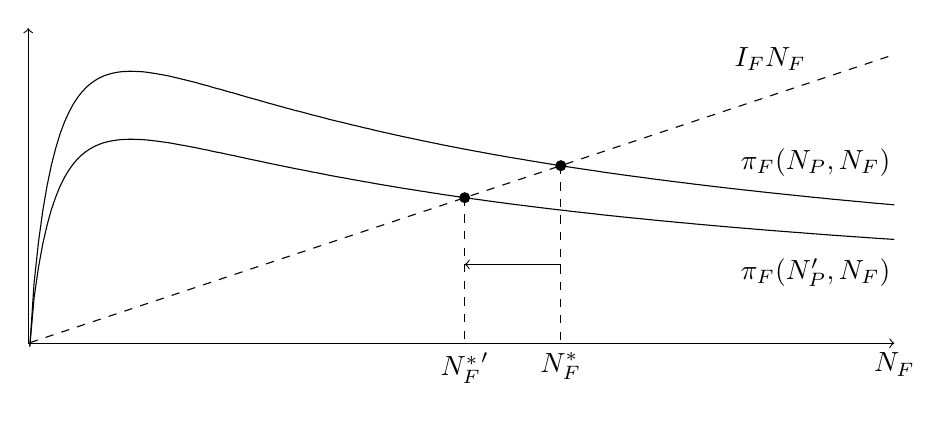
\begin{tikzpicture}[xscale=2,yscale=2,samples=200]
        \draw[->] (0,0) -- (0,2);
        \draw[->] (0,0) -- (5.5,0) node[below] {$N_F$};

        \draw[name path=piF,domain=0.01:5.5,variable=\x,black] plot ({\x},{8*((\x)/(0.3+\x))-8*((\x-0.3*ln(\x+0.3)-0.361)/(\x))});
        \draw[name path=piF2,domain=0.01:5.5,variable=\x,black] plot ({\x},{6*((\x)/(0.3+\x))-6*((\x-0.3*ln(\x+0.3)-0.361)/(\x))});
        \draw[name path=IF,domain=0.01:5.5,variable=\x,black,dashed] plot ({\x},{(\x)/3});

        \node[anchor=south] at (5,1) {$\pi_F(N_P, N_F)$};
        \node[anchor=north] at (5,0.6) {$\pi_F(N_P', N_F)$};
        \node[anchor=south east] at (5,5/3) {$I_F N_F$};

        \fill [name intersections={of=piF and IF, name=i, total=\t}]
            [black] (i-2) circle (1pt);
        \draw[dashed] (i-2) -- (i-2 |- 0,0) node[below] {$N_F^*$};
        \fill [name intersections={of=piF2 and IF, name=i2, total=\t}]
            [black] (i2-2) circle (1pt);
        \draw[dashed] (i2-2) -- (i2-2 |- 0,0) node[below] {${N_F^*}'$};

        \draw[->] (i-2 |- 0,0.5) -- (i2-2 |- 0,0.5);
    \end{tikzpicture}
    \caption{Illustration of comparative statics for equilibrium entry. If the change in $N_P$ decreases the fringe's profits for every $N_F \geq 0$, then equilibrium can be restored by decreasing the number of fringe entrants.}
    \label{fig:comparative_N_F}
\end{figure}

When the fringe is not viable, the platform's product variety has the same, mechanical effect on total aggregate and consumer surplus as in the benchmark model.
\begin{proposition}
    \label{prop:aggregate_comparative_retail}
    Assume that the platform is operating in the pure retail regime. Then the equilibrium aggregate and consumer surplus is increasing in the number of the platform's products.
    \begin{align*}
        N_F = 0 \implies \frac{\partial A}{\partial N_P}, \frac{\partial CS}{\partial N_P} > 0.
    \end{align*}
\end{proposition}
This set of results is in stark contrast to the benchmark model.
Instead of increased product variety weakly increasing consumer welfare, when entry fees are negotiated, it can actually decrease it if the platform stays in the hybrid regime.

This conclusion is in line with many of the findings in the literature on hybrid platforms, such as \textcite{hagiu2022should} or \textcite{anderson2021hybrid}.
The channel through which this happens, and thus the potential policy implications, are quite different, however.
In \textcite{hagiu2022should}, the negative consequences are due to its incentives to engage in anti-competitive behavior, such as self-preferencing or imitation.
In their model, in the absence of such behavior, hybrid platforms can actually increase consumer welfare.
\textcite{anderson2021hybrid}, on the other hand, shows that even in the absence of such behavior, hybrid platforms can harm consumers, as platforms are inclined to set higher than optimal royalties to create a price advantage for their own products.
This model goes one step further.
Due to the lump-sum nature of the entry fee and platforms pricing their products as if they were produced by separate sellers, this inventive is no more present (as demonstrated by the benchmark model).
However, the fact that the platform having its own products improves its bargaining position leads to a different distortion: the platform sets higher entry fees than it would if it had no products on its own.

\subsection{Example and comparison}

In this section, I look a specific example to illustrate the main results and compare the benchmark and bargaining models.
But first, let us collect and state the most important results from the previous sections in one theorem each for both models.

In the benchmark model, the platform having its own product variety has a weakly positive effect.
As long as the market is in the hybrid regime, and there is a non-zero number of fringe firms, it has no effect on the aggregate or consumer surplus.
When the fringe is no longer feasible, and the platform is in the pure retail regime, the platform's product variety mechanically increases both.
\begin{theorem}
    \label{prop:benchmark_results}
    In the benchmark model with unilateral price setting, in a hybrid regime equilibrium (with $N_F > 0$), the following results hold:
    \begin{itemize}
        \item The equilibrium number of fringe firms decreases in the number of the platform's products: $\frac{\partial N_F}{\partial N_P} = -\frac{V_P}{V_F} < 0$.
        \item The aggregate is independent of the platform's product variety: $\frac{\partial A}{\partial N_P} = 0$.
        \item Consumer surplus is independent of the platform's product variety: $\frac{\partial CS}{\partial N_P} = 0$.
        % \item The platform's profit is increasing in the number of its products: $\frac{\partial \pi_P^t}{\partial N_P} = \frac{V_P}{V_F} I_F$.
    \end{itemize}
\end{theorem}

In contrast, in the bargaining model, increasing the platform's product variety can have a negative effect on consumer welfare.
The reason for this is that the platform's product variety increases its bargaining power, and thus decreases the share that the fringe firms obtain.
This in turn leads to a decrease in the number of fringe firms, and this decrease is large enough to offset the increase in the platform's product variety.
\begin{theorem}
    \label{prop:bargaining_results}
    In the bargaining model, in a hybrid regime equilibrium (with $N_F > 0$), the following results hold:
    \begin{itemize}
        \item The equilibrium number of fringe firms decreases in the number of the platform's products more than in the benchmark case: $\frac{\partial N_F}{\partial N_P} < -\frac{V_P}{V_F} 0$.
        \item The aggregate decreases in the platform's product variety: $\frac{\partial A}{\partial N_P} < 0$.
        \item Consumer surplus decreases in the platform's product variety: $\frac{\partial CS}{\partial N_P} < 0$.
    \end{itemize}
\end{theorem}

The statements of these theorems are illustrated in \cref{fig:comparative_N_F} and \cref{fig:welfare_aggregate} and \cref{fig:platform_profits}.
The intuition behind these results can be demonstrated by looking at entry fees.
First, define the implied entry fee in the bargaining case as the difference between the variable profit and the final, total profit of the fringe firms (bar the investment cost):
\begin{align*}
    K_F^{\text{impl}} = \pi_F^v - \pi_F^t.
\end{align*}
As shown before, as the platform's product variety grows, its bargaining power also increases.
This can be thought of as an increase in (implied) entry fees $K_F^{\text{impl}}$, which in turn discourages fringe entry.
This is not happening in the benchmark model, as the optimal entry fee does not depend on the platform's product variety.
\Cref{fig:entry_fee} demonstrates this effect.

In the example parametrization, the implied entry fee is lower than what the platform would prefer to set for low values of $N_P$, and higher afterwards.
There is an optimal platform product variety $N_P^*$ for which the implied entry fee is the same as the optimal entry fee in the benchmark model, and therefore the results of the two models are the same.
For $N_P > N_P^*$, the platform would like to commit to a lower entry fee to incentivize more fringe entry.
This is an example that bargaining instead of unilateral pricing does not necessarily lead to lower platform shares, or better welfare outcomes: it can be a lose-lose situation for both the platform and the consumers.

Finally, let us look at the platform's profits in equilibrium.
As in the benchmark model, they are increasing in the number platform's product variety $N_P$ (\cref{fig:platform_profits}). % TODO: can I make it a proper proposition?
However, in contrast to that case, there is an important difference in the hybrid regime.
In the benchmark model, the entry fee was independent of the platform's product variety.
On the other hand, with bargaining, it is increasing in $N_P$ (\cref{fig:entry_fee}).
Therefore, if the entry fee is lower than optimal, then the increase in $N_P$ will bring it closer to the optimal level, and the increase in platform profits will be higher than in the benchmark model.
On the other hand, when the entry fee is already higher than optimal for a given $N_P$, an additional increase will lead to an even more suboptimal (implied) entry fee, and thus a lower increase in platform profits.

% This means that, if the platform had to create its product variety at a per-unit investment cost of $I_P$, it would make different (inefficient) choices compared to the benchmark model.
% In particular, it might invest in some products even if it has a product disadvantage, and it might not invest in some products even if it has a product disadvantage.
% This phenomenon is more pronounced when the implied entry fee for $N_P = 0$ is lower than optimal, and is explored in more detail in \cref{sec:lower_bargaining_power}.

\begin{figure}
    \centering
    \begin{subfigure}[b]{0.45\textwidth}
        \centering
        \begin{tikzpicture}
            \begin{axis}[
                    xlabel={$N_P$},
                    xmin=0, xmax=4.5, % adjust these values as needed
                    ymin=0, ymax=4.4, % adjust these values as needed
                    width=\linewidth, % adjust the width of the plot
                    axis lines=left,
                    xtick={0, 4.5},
                ]
                \addplot[color=myblue,mark=none,thick] table[x=N_P,y=N_F_bench]{\equilibrium};
                \addplot[color=myred,mark=none,thick] table[x=N_P,y=N_F]{\equilibrium};
                \legend{Benchmark, Bargaining}

                \addplot[draw=none,name path=hybrid] table[x=N_P,y=hybrid]{\equilibrium};
                \addplot[draw=none,name path=hybrid_bench] table[x=N_P,y=hybrid_bench]{\equilibrium};
                \addplot[draw=none,name path=bottom] {0};
                \addplot [fill=black, fill opacity=0.05] fill between [of=hybrid and bottom];
                \addplot [fill=black, fill opacity=0.05] fill between [of=hybrid_bench and bottom];
            \end{axis}
        \end{tikzpicture}
        \caption{Equilibrium number of fringe firms ($N_F$)}
        \label{fig:fringe_entry_eq}
    \end{subfigure}
    \hfill
    \begin{subfigure}[b]{0.45\textwidth}
        \centering
        \begin{tikzpicture}
            \begin{axis}[
                    xlabel={$N_P$},
                    ylabel={$K_F$},
                    xmin=0, xmax=4.5, % adjust these values as needed
                    ymin=0, ymax=0.35, % adjust these values as needed
                    width=\linewidth, % adjust the width of the plot
                    axis lines=left,
                    xtick={0, 4.5},
                    legend pos=south east
                ]
                \addplot[color=myblue,mark=none,thick] table[x=N_P,y=K_F_opt]{\equilibrium};
                \addplot[color=myred,mark=none,thick] table[x=N_P,y=K_F_implied]{\equilibrium};
                \legend{Benchmark, Bargaining (implied)}

                \addplot[draw=none,name path=hybrid] table[x=N_P,y=hybrid]{\equilibrium};
                \addplot[draw=none,name path=hybrid_bench] table[x=N_P,y=hybrid_bench]{\equilibrium};
                \addplot[draw=none,name path=bottom] {0};
                \addplot [fill=black, fill opacity=0.05] fill between [of=hybrid and bottom];
                \addplot [fill=black, fill opacity=0.05] fill between [of=hybrid_bench and bottom];
            \end{axis}
        \end{tikzpicture}
        \caption{Optimal/implied entry fee ($K_F$)}
        \label{fig:entry_fee}
    \end{subfigure}
    \caption{Equilibrium number of fringe entrants and (implied) entry fees ($\mu = 1, N_C = 1, V_P = 1, V_F = 1, I_F = 0.05$). In the benchmark model, the entry fee does not depend on the platform's product variety, and an increase in $N_P$ leads to a proportional reduction in $N_F$. In contrast, in the bargaining case, the entry fee is increasing in $N_P$, and the reduction in $N_F$ is more than proportional. Dark shaded area represents hybrid mode under the bargaining assumption, while light shaded area represents additional hybrid mode under the benchmark assumption.}
    \label{fig:entry_and_fees}
\end{figure}


\begin{figure}
    \centering
    \begin{subfigure}[b]{0.45\textwidth}
        \centering
        \begin{tikzpicture}
            \begin{axis}[
                    xlabel={$N_P$},
                        xmin=0, xmax=4.5, % adjust these values as needed
                        ymin=0, ymax=0.9, % adjust these values as needed
                        width=\linewidth, % adjust the width of the plot
                        axis lines=left,
                        xtick={0, 4.5},
                        legend pos=south east
                    ]
                \addplot[color=myblue,mark=none,thick] table[x=N_P,y=pi_P_bench]{\equilibrium};
                \addplot[color=myred,mark=none,thick] table[x=N_P,y=pi_P]{\equilibrium};
                \addplot[color=black,mark=none,thick,dashed] table[x=N_P,y=pi_P_noF]{\equilibrium};
                \legend{Benchmark, Bargaining, Pure retail}

                \addplot[draw=none,name path=hybrid] table[x=N_P,y=hybrid]{\equilibrium};
                \addplot[draw=none,name path=hybrid_bench] table[x=N_P,y=hybrid_bench]{\equilibrium};
                \addplot[draw=none,name path=bottom] {0};
                \addplot [fill=black, fill opacity=0.05] fill between [of=hybrid and bottom];
                \addplot [fill=black, fill opacity=0.05] fill between [of=hybrid_bench and bottom];
            \end{axis}
        \end{tikzpicture}
        \caption{}
    \end{subfigure}
    \hfill
    \begin{subfigure}[b]{0.45\textwidth}
        \centering
        \begin{tikzpicture}
            \begin{axis}[
                    xlabel={$N_P$},
                        xmin=0, xmax=1, % adjust these values as needed
                        ymin=0.58, ymax=0.67, % adjust these values as needed
                        width=\linewidth, % adjust the width of the plot
                        axis lines=left,
                        xtick={0, 1},
                        legend pos=south east
                    ]
                \addplot[color=myblue,mark=none,thick] table[x=N_P,y=pi_P_bench]{\equilibrium};
                \addplot[color=myred,mark=none,thick] table[x=N_P,y=pi_P]{\equilibrium};
                \legend{Benchmark, Bargaining}

                \addplot[draw=none,name path=hybrid] table[x=N_P,y=hybrid]{\equilibrium};
                \addplot[draw=none,name path=hybrid_bench] table[x=N_P,y=hybrid_bench]{\equilibrium};
                \addplot[draw=none,name path=bottom] {0};
                \addplot [fill=black, fill opacity=0.05] fill between [of=hybrid and bottom];
                \addplot [fill=black, fill opacity=0.05] fill between [of=hybrid_bench and bottom];
            \end{axis}
        \end{tikzpicture}
        \caption{}
    \end{subfigure}
    \caption{Platform profits in equilibrium ($\mu = 1, N_C = 1, V_P = 1, V_F = 1, I_F = 0.05$). In both cases, platform profits are increasing in $N_P$. In the case of the hybrid regime under bargaining, this increase is higher than in the benchmark case as long as the implied the entry fee is lower than optimal, and lower afterwards. The right-hand side graph zooms on the relevant section to highlight this observation. Dark shaded area represents hybrid mode under the bargaining assumption, while light shaded area represents additional hybrid mode under the benchmark assumption.}
    \label{fig:platform_profits}
\end{figure}

\begin{figure}
    \centering
    \begin{subfigure}[b]{0.45\textwidth}
        \centering
        \begin{tikzpicture}
            \begin{axis}[
                    xlabel={$N_P$},
                    xmin=0, xmax=4.5, % adjust these values as needed
                    ymin=0, ymax=5.8, % adjust these values as needed
                    width=\linewidth, % adjust the width of the plot
                    axis lines=left,
                    xtick={0, 4.5},
                    legend pos=south east
                ]
                \addplot[color=myblue,mark=none,thick] table[x=N_P,y=A_bench]{\equilibrium};
                \addplot[color=myred,mark=none,thick] table[x=N_P,y=A]{\equilibrium};
                \addplot[color=black,mark=none,thick,dashed] table[x=N_P,y=A_noF]{\equilibrium};
                \legend{Benchmark, Bargaining, Pure retail}

                \addplot[draw=none,name path=hybrid] table[x=N_P,y=hybrid]{\equilibrium};
                \addplot[draw=none,name path=hybrid_bench] table[x=N_P,y=hybrid_bench]{\equilibrium};
                \addplot[draw=none,name path=bottom] {0};
                \addplot [fill=black, fill opacity=0.05] fill between [of=hybrid and bottom];
                \addplot [fill=black, fill opacity=0.05] fill between [of=hybrid_bench and bottom];
            \end{axis}
        \end{tikzpicture}
        \caption{Aggregate ($A$)}
        \label{fig:welfare_aggregate}
    \end{subfigure}
    \hfill
    \begin{subfigure}[b]{0.45\textwidth}
        \centering
        \begin{tikzpicture}
            \begin{axis}[
                    xlabel={$N_P$},
                    xmin=0, xmax=4.5, % adjust these values as needed
                    ymin=0, ymax=2, % adjust these values as needed
                    width=\linewidth, % adjust the width of the plot
                    axis lines=left,
                    xtick={0, 4.5},
                    legend pos=south east
                ]
                \addplot[color=myblue,mark=none,thick] table[x=N_P,y=CS_bench]{\equilibrium};
                \addplot[color=myred,mark=none,thick] table[x=N_P,y=CS]{\equilibrium};
                \addplot[color=black,mark=none,thick,dashed] table[x=N_P,y=CS_noF]{\equilibrium};
                \legend{Benchmark, Bargaining, Pure retail}

                \addplot[draw=none,name path=hybrid] table[x=N_P,y=hybrid]{\equilibrium};
                \addplot[draw=none,name path=hybrid_bench] table[x=N_P,y=hybrid_bench]{\equilibrium};
                \addplot[draw=none,name path=bottom] {0};
                \addplot [fill=black, fill opacity=0.05] fill between [of=hybrid and bottom];
                \addplot [fill=black, fill opacity=0.05] fill between [of=hybrid_bench and bottom];
            \end{axis}
        \end{tikzpicture}
        \caption{Consumer surplus ($CS$)}
        \label{fig:welfare_consumer_surplus}
    \end{subfigure}
    \caption{Size of the aggregate and consumer surplus in equilibrium ($\mu = 1, N_C = 1, V_P = 1, V_F = 1, I_F = 0.05$). In the benchmark model, an increase in platform product variety has no effect in the hybrid regime. Under bargaining, it does have a negative effect on total product variety, and, in turn, consumer surplus. The increase has a (mechanical) positive effect in the pure retail regime under both assumptions. Dark shaded area represents hybrid mode under the bargaining assumption, while light shaded area represents additional hybrid mode under the benchmark assumption.}
    \label{fig:welfare}
\end{figure}


\section{Extensions}
\label{sec:extensions}

\subsection{Players have different innate bargaining power}
\label{sec:lower_bargaining_power}

In the previous sections, I assumed that the platform and the fringe firms split total profits according to their Shapley values.
Because of the symmetry property of the Shapley value, this excludes the possibility of players having some kind of innate bargaining power, which is not related to their profit functions.
In this extension, I will relax this assumption, and assume instead that profits are shared according to \emph{weighed} values.
These are a generalization of the Shapley value, where each player has a weight $w_i$ that can, in certain settings, be thought of as a parameter describing bargaining power.\footnote{
    \textcite{hart1996bargaining} and \textcite{stole1996intra} provide foundations for this interpretation.
}
I still assume that fringe firms are identical, also in regard to their bargaining weights.
Therefore, the only difference is between the platform and the fringe firms.
Let us denote the platform's bargaining weight as $\lambda_P \in \mathbb{R}^+$, and without loss of generality, normalize the fringe firms' weights to 1.

As shown in \cref{sec:cooperative_game_weighted}, the weighted Shapley value, and thus final profits in this setting is given by
\begin{proposition}
    \label{prop:weighted_shapley_value}
    The Shapley value of the platform and the fringe firms, and thus final total profits, are given by:
    \begin{align*}
        \pi^t_P(N_P, N_F) &= N_C \int_0^1 \lambda_P s ^ {\lambda_P - 1} \Pi(N_P,s N_F) \ds, \\
        \pi^t_F(N_P, N_F) &= N_C \int_0^1 s ^ {\lambda_P} \partial_2 N_F \Pi(N_P,s N_F) \ds.
    \end{align*}
\end{proposition}
It is similar to the non-weighted value in that it is an average of marginal contributions, but now those averages are weighted, with the weight function depending on platform's bargaining weight.

The interpretation of $\lambda_P$ as a bargaining weight for the platform is supported by the fact that the platform's profit function is increasing in it.
\begin{proposition}
    \label{prop:lambda_P_comparative}
    For any fixed $N_F >0, N_P \geq 0$, the platform's total profits are increasing in its bargaining weight $\lambda_P$, while the fringe's profits are decreasing in it:
    \begin{align*}
        \frac{\partial \pi_P^t(N_P, N_F)}{\partial \lambda_P} &> 0, \\
        \frac{\partial \pi_F^t(N_P, N_F)}{\partial \lambda_P} &< 0.
    \end{align*}
\end{proposition}
In fact, the limits as $\lambda_P \to 0$ and $\lambda_P \to \infty$ are quite intuitive: in the former case, the platform's profits are zero, while in the latter case it is able to appropriate all profits.
That is, these limits correspond to the platform either receiving or making take-it or leave-it offers.

\textcolor{red}{TODO: can I show a result analogous to \cref{lem:shape_of_fringe_profit} still holds for any $\lambda_P$? If not, focus on a specific case, such as the one on the graphs.}

The example parametrizatrion is the same as in the main model, with the only difference that the platform has a higher innate bargaining power ($\lambda_P = 2$).
The main result, namely that the platform's product variety has a negative effect on consumer welfare in the hybrid regime, still holds.
That is, as shown on \cref{fig:fringe_entry_eq_high_lambda}, total aggregate is decreasing in $N_P$ throughout the hybrid regime, due to the platform's products displacing more fringe products than their total number.

The main difference is that, for any $N_P\geq 0$, the implied entry fee (\cref{fig:platform_profits_high_lambda}) is higher than the benchmark, unilaterally set one,  due to the higher bargaining power of the platform.
That is, for any $N_P$, the platform would prefer to set a lower entry fee, but it is unable to do so due to its high bargaining power.
Total aggregate, and thus consumer surplus, is also below the main model's outcome in this case.

Another major difference pertains to the total profits of the platform as a function of $N_P$.
It is still true that they are increasing in the number of the platform's products, but now this increase is even slower in the hybrid regime.
The reason is that the implied entry fee is always higher than the optimal one, therefore an increase the positive effect of an increase in $N_P$ is somewhat counterbalanced by the entry fee becoming even more suboptimal.

\Cref{fig:equilibrium_high_lambda_entry_fees} demonstrates an important consequence of this phenomenon.
Imagine that the platform can decide on the number of its products at time 0, at an investment cost of $I_P$ per product.
In the example for the main model, due to the implied entry fee being higher than optimal even for $N_P = 0$, hybrid operation may be optimal for certain values of $I_P$ (most notably, $I_P = I_F = 0.05$).
In contrast, in the example with the platform having higher bargaining power, it would always prefer either pure retail or pure marketplace operation.

\begin{figure}
    \centering
    \begin{subfigure}[b]{0.45\textwidth}
        \centering
        \begin{tikzpicture}
            \begin{axis}[
                    xlabel={$N_P$},
                    xmin=0, xmax=4.5, % adjust these values as needed
                    ymin=0, ymax=4.4, % adjust these values as needed
                    width=\linewidth, % adjust the width of the plot
                    axis lines=left,
                    xtick={0, 4.5},
                ]
                \addplot[color=myblue,mark=none,thick] table[x=N_P,y=N_F_bench]{\equilibrium};
                \addplot[color=myred,mark=none,thick] table[x=N_P,y=N_F]{\equilibrium};
                \addplot[color=mygreen,mark=none,thick] table[x=N_P,y=N_F]{\equilibriumProfitOneSidedHighLambda};
                \legend{Benchmark, Bargaining ($\lambda = 1$), Bargaining ($\lambda = 2$)}

                \addplot[draw=none,name path=hybrid] table[x=N_P,y=hybrid]{\equilibrium};
                \addplot[draw=none,name path=hybrid_alt] table[x=N_P,y=hybrid]{\equilibriumProfitOneSidedHighLambda};
                \addplot[draw=none,name path=bottom] {0};
                \addplot [fill=black, fill opacity=0.05] fill between [of=hybrid and bottom];
                \addplot [fill=black, fill opacity=0.05] fill between [of=hybrid_alt and bottom];
            \end{axis}
        \end{tikzpicture}
        \caption{Equilibrium number of fringe firms ($N_F$)}
        \label{fig:fringe_entry_eq_high_lambda}
    \end{subfigure}
    \hfill
    \begin{subfigure}[b]{0.45\textwidth}
        \centering
        \begin{tikzpicture}
            \begin{axis}[
                    xlabel={$N_P$},
                    xmin=0, xmax=4.5, % adjust these values as needed
                    ymin=0, ymax=2, % adjust these values as needed
                    width=\linewidth, % adjust the width of the plot
                    axis lines=left,
                    xtick={0, 4.5},
                    legend pos=south east,
                ]
                \addplot[color=myblue,mark=none,thick] table[x=N_P,y=CS_bench]{\equilibrium};
                \addplot[color=myred,mark=none,thick] table[x=N_P,y=CS]{\equilibrium};
                \addplot[color=mygreen,mark=none,thick] table[x=N_P,y=CS]{\equilibriumProfitOneSidedHighLambda};
                \legend{Benchmark, Bargaining ($\lambda = 1$), Bargaining ($\lambda = 2$)}

                \addplot[draw=none,name path=hybrid] table[x=N_P,y=hybrid]{\equilibrium};
                \addplot[draw=none,name path=hybrid_alt] table[x=N_P,y=hybrid]{\equilibriumProfitOneSidedHighLambda};
                \addplot[draw=none,name path=bottom] {0};
                \addplot [fill=black, fill opacity=0.05] fill between [of=hybrid and bottom];
                \addplot [fill=black, fill opacity=0.05] fill between [of=hybrid_alt and bottom];
            \end{axis}
        \end{tikzpicture}
        \caption{Equilibrium consumer surplus ($CS$)}
    \end{subfigure}
    \caption{Equilibrium outcomes in the case when the platform has higher innate bargaining power ($N_C = 1, V_P = 1, V_F = 1, I_F = 0.05$). As before, consumer surplus is decreasing in $N_P$ as a result in a decrease in total product variety. Dark shaded area represents hybrid mode under $\lambda=2$, while light shaded area represents additional hybrid mode under $\lambda=1$.}
    \label{fig:equilibrium_high_lambda}
\end{figure}


\begin{figure}
    \centering
    \begin{subfigure}[b]{0.45\textwidth}
        \centering
        \begin{tikzpicture}
            \begin{axis}[
                    xlabel={$N_P$},
                    ylabel={},
                    xmin=0, xmax=4.5, % adjust these values as needed
                    ymin=0, ymax=0.9, % adjust these values as needed
                    axis lines=left,
                    xtick={0, 4.5},
                    legend pos=south east,
                    width=\linewidth,
                ]
                \addplot[color=myblue,mark=none,thick] table[x=N_P,y=pi_P_bench]{\equilibrium};
                \addplot[color=myred,mark=none,thick] table[x=N_P,y=pi_P]{\equilibrium};
                \addplot[color=mygreen,mark=none,thick] table[x=N_P,y=pi_P]{\equilibriumProfitOneSidedHighLambda};
                \addplot[color=black,mark=none,thick,dashed] table[x=N_P,y=pi_P_noF]{\equilibrium};

                \legend{Benchmark, Bargaining ($\lambda = 1$), Bargaining ($\lambda = 2$)}
                
                \addplot[draw=none,name path=hybrid] table[x=N_P,y=hybrid]{\equilibriumProfitOneSidedHighLambda};
                \addplot[draw=none,name path=hybrid_orig] table[x=N_P,y=hybrid]{\equilibrium};
                \addplot[draw=none,name path=bottom] {0};
                \addplot [fill=black, fill opacity=0.05] fill between [of=hybrid and bottom];
                \addplot [fill=black, fill opacity=0.05] fill between [of=hybrid_orig and bottom];
            \end{axis}
        \end{tikzpicture}
        \caption{Platform profits}
        \label{fig:platform_profits_high_lambda}
    \end{subfigure}
    \hfill
    \begin{subfigure}[b]{0.45\textwidth}
        \centering
        \begin{tikzpicture}
            \begin{axis}[
                    xlabel={$N_P$},
                    ylabel={},
                    xmin=0, xmax=4.5, % adjust these values as needed
                    ymin=0, ymax=0.4, % adjust these values as needed
                    axis lines=left,
                    xtick={0, 4.5},
                    legend pos=south east,
                    width=\linewidth,
                ]
                \addplot[color=myblue,mark=none,thick] table[x=N_P,y=K_F_opt]{\equilibrium};
                \addplot[color=myred,mark=none,thick] table[x=N_P,y=K_F_implied]{\equilibrium};
                \addplot[color=mygreen,mark=none,thick] table[x=N_P,y=K_F_implied]{\equilibriumProfitOneSidedHighLambda};

                \legend{Benchmark, Bargaining ($\lambda = 1$), Bargaining ($\lambda = 2$)}
                
                \addplot[draw=none,name path=hybrid] table[x=N_P,y=hybrid]{\equilibriumProfitOneSidedHighLambda};
                \addplot[draw=none,name path=hybrid_orig] table[x=N_P,y=hybrid]{\equilibrium};
                \addplot[draw=none,name path=bottom] {0};
                \addplot [fill=black, fill opacity=0.05] fill between [of=hybrid and bottom];
                \addplot [fill=black, fill opacity=0.05] fill between [of=hybrid_orig and bottom];
            \end{axis}
        \end{tikzpicture}
        \caption{Optimal/implied entry fee}
        \label{fig:entry_fee_high_lambda}
    \end{subfigure}
    \caption{Platform profits and (implied) entry fees ($\mu = 0.2, N_C = 1, V_P = 1, V_F = 1, I_F = 0.05$). Regardless of lambda, platform profits and entry fees are increasing in $N_P$. However, when the platform's innate bargaining power is higher, entry fees are above optimal levels already for $N_P = 0$, and the additional increase somewhat mitigates the benefits of the platform's increased product variety. When $\lambda$ is lower, the entry fees are below optimal for low $N_P$, therefore increasing $N_P$ has a larger positive effect on profits. Dark shaded area represents hybrid mode under $\lambda=2$, while light shaded area represents additional hybrid mode under $\lambda=1$.}
    \label{fig:profits_and_entry_fees_high_lambda}
\end{figure}


\begin{figure}
    \centering
    \begin{subfigure}[b]{0.45\textwidth}
        \centering
        \begin{tikzpicture}
            \begin{axis}[
                    xlabel={$N_P$},
                    ylabel={},
                    xmin=0, xmax=4.5, % adjust these values as needed
                    ymin=0.2, ymax=0.7, % adjust these values as needed
                    axis lines=left,
                    xtick={0, 4.5},
                    legend pos=south west,
                    width=\linewidth,
                ]
                \addplot[color=myblue,mark=none,thick] table[x=N_P,y expr=\thisrow{pi_P} - \thisrow{N_P} * 0.04]{\equilibrium};
                \addplot[color=myred,mark=none,thick] table[x=N_P,y expr=\thisrow{pi_P} - \thisrow{N_P} * 0.05]{\equilibrium};
                \addplot[color=mygreen,mark=none,thick] table[x=N_P,y expr=\thisrow{pi_P} - \thisrow{N_P} * 0.06]{\equilibrium};

                \addplot[draw=none,name path=hybrid] table[x=N_P,y=hybrid]{\equilibrium};
                \addplot[draw=none,name path=bottom] {0};
                \addplot [fill=black, fill opacity=0.05] fill between [of=hybrid and bottom];

                \legend{$I_P = 0.04$, $I_P = 0.05$, $I_P = 0.05$}
            \end{axis}
        \end{tikzpicture}
        \caption{$\lambda = 1$}
    \end{subfigure}
    \hfill
    \begin{subfigure}[b]{0.45\textwidth}
        \centering
        \begin{tikzpicture}
            \begin{axis}[
                    xlabel={$N_P$},
                    ylabel={},
                    xmin=0, xmax=4.5, % adjust these values as needed
                    ymin=0.2, ymax=0.7, % adjust these values as needed
                    axis lines=left,
                    xtick={0, 4.5},
                    legend pos=south west,
                    width=\linewidth,
                ]
                \addplot[color=myblue,mark=none,thick] table[x=N_P,y expr=\thisrow{pi_P} - \thisrow{N_P} * 0.04]{\equilibriumProfitOneSidedHighLambda};
                \addplot[color=myred,mark=none,thick] table[x=N_P,y expr=\thisrow{pi_P} - \thisrow{N_P} * 0.05]{\equilibriumProfitOneSidedHighLambda};
                \addplot[color=mygreen,mark=none,thick] table[x=N_P,y expr=\thisrow{pi_P} - \thisrow{N_P} * 0.06]{\equilibriumProfitOneSidedHighLambda};

                \addplot[draw=none,name path=hybrid] table[x=N_P,y=hybrid]{\equilibriumProfitOneSidedHighLambda};
                \addplot[draw=none,name path=bottom] {0};
                \addplot [fill=black, fill opacity=0.05] fill between [of=hybrid and bottom];

                \legend{$I_P = 0.04$, $I_P = 0.05$, $I_P = 0.05$}
            \end{axis}
        \end{tikzpicture}
        \caption{$\lambda = 0.5$}
    \end{subfigure}
    \caption{Total platform profits if the platform incurs an investment cost for creating its own products ($\pi_P(N_P) - I_P N_P$). In the high bargaining power case (right), the platform never chooses to operate in hybrid mode. It either becomes a pure marketplace or a pure retailer. In the case of lower $\lambda_P$ (left), choosing the hybrid mode can be optimal depending on $I_P$. The shaded region represents hybrid operation, while in the unshaded region, the platform operates in pure retail mode ($\mu = 1, N_C = 1, V_P = 1, V_F = 1, I_F = 0.05$).}
    \label{fig:equilibrium_high_lambda_entry_fees}
\end{figure}


\subsection{Consumers also participate in bargaining}
\label{sec:two_sided}

In the second extension, I consider the case when the consumers also participate in the bargaining process.
This entails two changes compared to the main model.
First, the players bargain over the total surplus generated on all sides of the market, not just total profits.
Second, the outcomes are assumed to be described by a cooperative game with three types of players: the platform, the fringe firms, and the consumers.

Let us start by deriving total surplus as a function of $N_P, N_F$ and $N_C$.
Under the logit-like demand structure described in \cref{sec:demand}, the total surplus is given by
\begin{proposition}
    \label{prop:profits_total_surplus}
    Assuming profit-maximizing prices from the platform and the fringe, total surplus as a function of $N_P, N_F$ and $N_C$ is given by
    \begin{align*}
        \Pi(N_P, N_F, N_C) = \mu N_C \left[ \frac{N_P V_P + N_F V_F}{N_P V_P + N_F V_F + 1} + \log(N_P V_P + N_F V_F + 1) \right].
    \end{align*}
\end{proposition}
\begin{proof}[Proof of \cref{prop:profits_total_surplus}]
    See \textcite{small1981applied} for a derivation for the discrete case.
    The continuous case is analogous.
\end{proof}
Note, that this expression is of the form $\Pi(N_P, N_P, N_C) = N_C f(N_P, N_F)$.
Furthermore, $f(N_P, N_F) = g(V_P N_P + V_F N_F)$ for an increasing, strictly concave $g$.

Next, let us consider the bargaining outcomes in this three-sided setting.
\Cref{sec:cooperative_game_two_sided} formally describes the corresponding cooperative game, and \cref{prop:profit_sharing_two_sided} establishes the resulting profit shares.
To summarize, the shares of the various players are as follows.
\begin{proposition}
    \label{prop:three_way_shapley_value}
    \begin{align*}
        \pi_P(N_P, N_F, N_C) &= \int_0^1 s \Pi(N_P, s N_F) \ds, \\
        \pi_F(N_P, N_F, N_C) &= \int_0^1 s^2 N_F \partial_2 \Pi(N_P, s N_F) \ds \\
        CS(N_P, N_F, N_C) &= \int_0^1 s \Pi(N_P, s N_F) \ds.
    \end{align*}
\end{proposition}

There are a number of things to note here.
First, and most importantly, the consumers' share from total surplus is equal to the platform's.\footnote{
    This is a consequence of the fact that the total surplus function is linear in the number of consumers.
}
As a consequence, what's good for the platform is also optimal for the consumers.
Therefore, if the platform can choose its mode of operation to maximize its profits, it maximizes consumer welfare, as well (but not necessarily total surplus).

Second, it can be shown that due to the fringe firms' total profit function having a similar shape as in the main model, the same results hold in terms of the platform's product variety displacing fringe products.
\begin{proposition}
    In the hybrid regime under three-sided bargaining, the following holds:
    \begin{align*}
        N_F > 0 \implies \frac{\partial N_F}{\partial N_P} < -\frac{V_P}{V_F}.
    \end{align*}
\end{proposition}
As a consequence, the aggregate is decreasing in $N_P$ in the hybrid regime (\cref{fig:fringe_entry_eq_full_surplus_two_sided}).
\begin{corollary}
    In the hybrid regime under three-sided bargaining, total aggregate is decreasing in the platform's product variety:
    \begin{align*}
        N_F > 0 \implies \frac{\partial A}{\partial N_P} < 0.
    \end{align*}
\end{corollary}

Nevertheless, there is an important distinction compared to the previous results.
While this does lead to a decrease in total surplus, in contrast to the two-sided bargaining case, this does not imply a decrease in consumer surplus.
As mentioned before, the consumers' share of total surplus is equal to the platform's profits, and thus it is increasing in $N_P$ if and only if platform profits (\cref{fig:profits_full_surplus_two_sided}) are.
Therefore, consumers might prefer hybrid operation to the platform being a pure marketplace.

\begin{figure}
    \centering
    \begin{subfigure}[b]{0.45\textwidth}
        \centering
        \begin{tikzpicture}
            \begin{axis}[
                    xlabel={$N_P$},
                    ylabel={},
                    xmin=0, xmax=4.5, % adjust these values as needed
                    ymin=0, ymax=7.5, % adjust these values as needed
                    axis lines=left,
                    xtick={0, 4.5},
                    legend pos=south east,
                    width=\linewidth,
                ]
                \addplot[color=myblue,mark=none,thick] table[x=N_P,y=N_P]{\equilibriumFullSurplusTwoSided};
                \addplot[color=myred,mark=none,thick] table[x=N_P,y=N_F]{\equilibriumFullSurplusTwoSided};
                \addplot[color=black,mark=none,thick] table[x=N_P,y=A]{\equilibriumFullSurplusTwoSided};
                
                \addplot[draw=none,name path=hybrid] table[x=N_P,y=hybrid]{\equilibriumFullSurplusTwoSided};
                \addplot[draw=none,name path=bottom] {0};
                \addplot [fill=black, fill opacity=0.05] fill between [of=hybrid and bottom];

                
                \legend{$N_P$, $N_F$, $A$}
            \end{axis}
        \end{tikzpicture}
        \caption{Platform product variety and number of fringe entrants}
        \label{fig:fringe_entry_eq_full_surplus_two_sided}
    \end{subfigure}
    \hfill
    \begin{subfigure}[b]{0.45\textwidth}
        \centering
        \begin{tikzpicture}
            \begin{axis}[
                    xlabel={$N_P$},
                    ylabel={},
                    xmin=0, xmax=4.5, % adjust these values as needed
                    ymin=0, ymax=1.2, % adjust these values as needed
                    axis lines=left,
                    xtick={0, 0.6},
                    legend pos=north west,
                    width=\linewidth,
                ]
                \addplot[color=myblue,mark=none,thick] table[x=N_P,y=pi_P]{\equilibriumFullSurplusTwoSided};
                \addplot[color=myred,mark=none,thick] table[x=N_P,y=pi_F]{\equilibriumFullSurplusTwoSided};
                \addplot[color=black,mark=none,thick,dashed] table[x=N_P,y=pi_P]{\equilibriumFullSurplusTwoSided};

                \addplot[draw=none,name path=hybrid] table[x=N_P,y=hybrid]{\equilibriumFullSurplusTwoSided};
                \addplot[draw=none,name path=bottom] {0};
                \addplot [fill=black, fill opacity=0.05] fill between [of=hybrid and bottom];

                \legend{$\pi_P$, $\pi_F$, $CS$}
            \end{axis}
        \end{tikzpicture}
        \caption{Platform and fringe profits}
        \label{fig:profits_full_surplus_two_sided}
    \end{subfigure}
    \caption{Equilibrium outcomes in the case when the whole surplus is bargained over ($N_C = 0.6, V_P = 1, V_F = 1, I_F = 0.05$), and both consumers and fringe firms participate in the bargaining. As before, the platform's profits are increasing in $N_P$, while the fringe's profits are decreasing. On the other hand, consumer welfare is equal to platform profits, therefore it is increasing in $N_P$. The shaded region represents hybrid operation, while in the unshaded region, the platform operates in pure retail mode.}
    \label{fig:equilibrium_full_surplus_two_sided}
\end{figure}

\section{Conclusion and future work}
\label{sec:conclusion}

This paper introduces a new model of hybrid platforms in which bargaining between the platform and the entrant firms plays a key role.
It highlights the importance of a so far overlooked aspect of platforms having their own products: the fact that it increases their bargaining power compared to other players'.
As a result, even in the absence of other frictions, hybrid platforms might have detrimental effects on fringe entry.
This, in certain situations, such as the one described in this paper, this can lead to fewer fringe reduced product variety, and ultimately, lower consumer welfare.

The contributions of this paper can be broken down into two categories.
First, a simple, but quite general model of bargaining between one indispensable player and a continuum of potential market entrants is introduced.
This model is applicable beyond the platform setting, and can describe other markets, such as upstream-downstream relations, or franchising, as well.
The quite general results obtained from this model also highlight the similarities between those markets.
Furthermore, many of the results from this paper can be applied in a plug-and-play fashion to other models of large-player-small-player interactions.

The second set of contributions pertains to applying the aforementioned model to a setting with a hybrid platform.
The demand structure is similar to the one in \textcite{anderson2021hybrid}, and the results convey the same general message: hybrid platforms can have detrimental welfare effects.
However, the mechanism behind this result is quite different.
This paper relies on the change in bargaing power, and shows that even in the case of lump-sum entry fees, hybrid platforms can be problematic from a welfare perspective.
An extension of the main model also highlight the importance of the assumptions on who is participating in the bargaining process.

There is a number of avenues for future research in this direction.
First, although the results provide some suggestions about what endogenizing the number of the platform's products might entail, a more formal analysis is needed for a more complete picture.
Second, applying the same bargaining framework, but using a different demand structure (e.g. CES utility) for microfounding the profit functions would have important implications for the robustness of the results.
Finally, I believe this approach for modeling bargaining is a rather good compromise between assuming that one party has all the bargaining power, and modeling the bargaining process in detail, and some of the main ideas in this paper might be a good fit for different settings and and more applied models.


\appendix

\printbibliography


\section{More general results}
\label{sec:more_general}

While the main text examines bargaining between the platform and the entrants in the context of a specific, logit-like demand system, many of the results are more general.
This section presents those and the necessary assumptions.
The proofs for many of the propositions in the main text also rely on these more general results.

\subsection{Production}
\label{sec:more_general_production}

Let us assume the following reduced-form, but rather general total profit (or, where applicable, surplus) function:
\begin{assumption}
    \label{ass:identical_fringe}
    The total profits of the platform and the fringe are described by 
    \begin{align*}
        \Pi(N_P, N_F, N_C) = N_C f(N_P, N_F),
    \end{align*}
    where $f: \mathbb{R}^+_0 \times \mathbb{R}^+_0 \to \mathbb{R}^+_0$.
\end{assumption}
It can be justified for markets with the following features: (1) all fringe firms are identical, thus only their number matters in terms of total profit, and (2) consumers are also identical (bar their idiosyncratic taste shocks).

I will assume that, in addition to being increasing in the number of consumers, total profits are also increasing in both the number of fringe firms and the platform' products.
\begin{assumption}
    \label{ass:monotone_profits}
    $f(n_P, n_F)$ is increasing in both $n_P$ and $n_F$.
\end{assumption}
Such profit functions arise in settings in which the profit reduction from increased competition is dominated by extra sales due to increased product variety.
One such example is \textcite{anderson2020aggregative}, where the demand exhibits love for variety, while consumers have access to an outside option.
Alternatively, indirect network effects, such as those in two-sided markets, can also result in such increasing profits.
Finally, if we assume that the platform can extract consumer surplus through entry fees or some similar mechanism, then this assumption will be true for any demand system in which total surplus is increasing in product variety.

\subsection{Profit sharing}
\label{sec:more_general_profit_sharing}
Next, assume that the platform and the fringe share profits according to the following rule:
\begin{assumption}
    \label{ass:profit_sharing}
    Let $w_P, w_F: \mathbb{R}^+_0 \to \mathbb{R}^+_0$ be non-negative functions such that the following condition holds: $\pi_P(N_P, N_F, N_C) + \pi_F(N_P, N_F, N_C) \leq \Pi(N_P, N_F, N_C)$.
    %TODO: can I make this condition nicer?
    Then, the platform's profit ($\pi_P(N_P, N_F, N_C)$) and the fringe's profit ($\pi_F(N_P, N_F, N_C)$) are given by:
    \begin{align*}
        \pi_P(N_P, N_F, N_C) &= N_C \int_0^1 w_P(s) f(N_P, s N_F) \ds, \\
        \pi_F(N_P, N_F, N_C) &= N_C \int_0^1 w_F(s) N_F \partial_2 f(N_P, s N_F) \ds.
    \end{align*}
\end{assumption}
It covers the cases in the main text (namely the Shapley value and the weighted value, and three-way bargaining), but is also more general than those.
In particular, in the platform game, any random order value \parencite{weber1988probabilistic} can be described by such a rule.

Apart from the cooperative foundations, one major justification for this profit allocation rule is its intuitive behavior in terms of comparative statistics.
To illustrate this, let us examine what happens when one varies the substitutability between the fringe firms.
As it turns out, the platform's share increases if the fringe firms are more substitutable.
The following observation demonstrates this idea.
\begin{proposition}
    \label{prop:outcome_based_bargaining_power}
    Fix some $N_P, N_C \geq 0$. Let $f, \tilde{f}: \mathbb{R}^+_0 \times \mathbb{R}^+_0 \to \mathbb{R}^+_0$ two different profit functions such that $f(N_P, N_F) = \tilde{f}(N_P, N_F)$ for some $N_P, N_F$ and $f(N_P, n_F) \leq \tilde{f}(N_P, n_F)$ for all $n_F < N_F$.
    Furthermore, let us denote the corresponding platform profit shares by $\pi_P$ and $\tilde{\pi}_P$.
    
    Then, $\pi_P \leq \tilde{\pi}_P$.
\end{proposition}

In words, \cref{prop:outcome_based_bargaining_power} describes two alternative worlds, in which $N_F$ fringe firms (assuming a platform with $N_P$ product variety and $N_C$ consumers) are able to achieve the same total profit level.
However, in one of these cases, the fringe firms are more substitutable to each other in the sense that fewer of them are needed to achieve a given level of profit (see \cref{fig:outcome_based_bargaining_power}).
The observation is that, in this situation, the platform's share is indeed higher when the fringe firms are more substitutable.
This coincides with the intuitive idea that the platform's bargaining power is higher when it does not really mind losing a few fringe sellers.

\begin{figure}
    \centering
    \begin{subfigure}[b]{0.45\textwidth}
        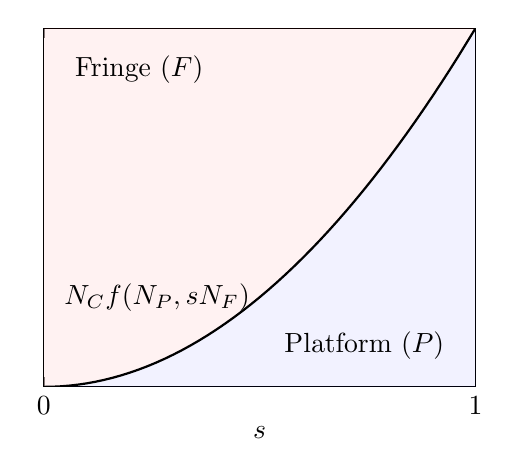
\begin{tikzpicture}[scale=0.8]
            \centering
            \begin{axis}[xmin=0, xmax=1, ymin=0, ymax=1, samples at={0, 0.02, ..., 0.98, 1},
                    xtick={0, 1}, ytick=\empty, xlabel={$s$}]
                \addplot[name path=f, black, thick] {x^2};
                \node[anchor= east] at (axis cs: .5, .5^2) {$N_C f(N_P, sN_F)$};
                \path[name path=bottom] (axis cs:0,0) -- (axis cs:1,0);
                \path[name path=top] (axis cs:0,1) -- (axis cs:1,1);
    
                \addplot [fill=blue, fill opacity=0.05] fill between [of=f and bottom];
                \addplot [fill=red, fill opacity=0.05] fill between [of=f and top];
    
                \node[anchor=north west] at (axis cs: .05, .95) {Fringe ($F$)};
                \node[anchor=south east] at (axis cs: .95, .05) {Platform ($P$)};
            \end{axis}
        \end{tikzpicture}
        \caption{Fringe firms are complements}
    \end{subfigure}
    \begin{subfigure}[b]{0.45\textwidth}
        \centering
        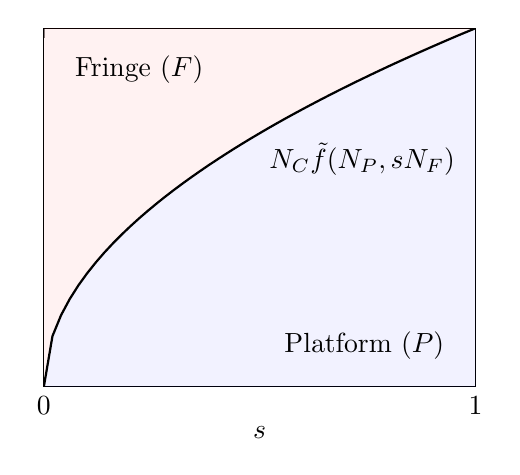
\begin{tikzpicture}[scale=0.8]
            \begin{axis}[xmin=0, xmax=1, ymin=0, ymax=1, samples at={0, 0.02, ..., 0.98, 1},
                xtick={0, 1}, ytick=\empty, xlabel={$s$}]
                \addplot[name path=f, black, thick] {x^0.5};
                \node[anchor=north west] at (axis cs: .5, .5^0.5) {$N_C \tilde{f}(N_P, sN_F)$};
                \path[name path=bottom] (axis cs:0,0) -- (axis cs:1,0);
                \path[name path=top] (axis cs:0,1) -- (axis cs:1,1);
    
                \addplot [fill=blue, fill opacity=0.05] fill between [of=f and bottom];
                \addplot [fill=red, fill opacity=0.05] fill between [of=f and top];
    
                \node[anchor=north west] at (axis cs: .05, .95) {Fringe ($F$)};
                \node[anchor=south east] at (axis cs: .95, .05) {Platform ($P$)};
            \end{axis}
        \end{tikzpicture}
        \caption{Fringe firms are substitutes}
    \end{subfigure}
    \caption{Distribution of value between the platform and the fringe. Profit shares correspond to the shaded areas. The platform's profit share is higher when the fringe firms are more substitutable.}
    \label{fig:outcome_based_bargaining_power}
\end{figure}

\subsection{Equilibrium}
\label{sec:more_general_equilibrium}

Let us now turn to the determination of the equilibrium number of fringe firms.
Assume that total investment cost for the fringe is given by some increasing, weakly convex function $I_F(N_F)$.
Note, that it includes the linear (per-firm constant) investment cost used throughout the main text.
\begin{assumption}
    Assume that $I_F(N_F)$ is a strictly increasing, convex, twice differentiable function:
    \begin{align*}
        \frac{\partial I_F(N_F)}{\partial N_F} > 0, \quad \frac{\partial^2 I_F(N_F)}{\partial N_F^2} \geq 0.
    \end{align*}
\end{assumption}

The equilibrium number of entrants is determined by a free entry condition: in the end, the fringe firms' total profits should be equal to the aggregated investment cost.
\begin{assumption}
    \label{ass:free_entry}
    Let us define a free entry equilibrium by the following conditions: Entrants make zero profits after accounting for entry costs: 
    \begin{align*}
        \pi_F(N_P, N_F) = I_F(N_F).
    \end{align*}
\end{assumption}

Finally, in order to guarantee a unique equilibrium, let us make the following, an additional assumption about the profit function.
\begin{assumption}
    \label{ass:single_crossing}
    Let $f$ be such that the following holds for all $N_F, N_P, N_C \geq 0$:
    \begin{align*}
        \frac{\partial \pi_F(N_P, N_F, N_C)}{\partial N_F} < 0 \text{ or } \frac{\partial^2 \pi_F(N_P, N_F, N_C)}{\partial N_F^2} < 0
    \end{align*}
\end{assumption}
This assumption essentially guarantees that the profit of the fringe (as a function of the number of entrants) has at most a single crossing with total entry cost (apart from the obvious $N_F=0$ intersection).
Again, the profit functions presented in the main text satisfy this assumption.

\subsection{Results}
\label{sec:more_general_results}

This section presents a number of results that can be derived even in this rather abstract setting.
Let us start with a technical, but very useful result.
\begin{proposition}
    \label{prop:unique_equilibrium_more_general}
    Under the conditions in \cref{ass:single_crossing}, the equilibrium is unique if it exists.
\end{proposition}
The intuition behind this result is that \cref{ass:single_crossing} ensures that the total profits achieved by the fringe is either concave or hump-shaped.
Consequently, it has at most one crossing with the -- convex and increasing -- total entry cost function (for $n_F > 0$).
This particular shape (concave or hump-shaped) is also the main driver for the later results about the comparative statics of equilibrium profits and entry.

The following two propositions are partial equilibrium results: consider the number of fringe entrants $N_F$ as fixed.
The first statement claims that the platform's profits are increasing in its own product variety.
\begin{proposition}
    \label{prop:share_of_platform}
    Assume that $f$ is continuously differentiable with respect to $N_P$ and also twice differentiable.
    Let $N_F \geq 0$.
    Then $\pi_P$ is also differentiable and
    \begin{align*}
        \frac{\partial \pi_P(N_P, N_F)}{\partial N_P} > 0.
    \end{align*}
\end{proposition}
While it might seem obvious, let us still examine what this result does and does not mean.
First, remember that $f$ is increasing in both arguments, and $N_F$ is fixed.
Therefore, an increase in $N_P$ also increases the size of the pie the participants bargain over.
This result states that the slice of the pie that the platform gets increases in this case, too.
It does not mean, however, that the \emph{relative share} of the pie that the platform gets is also bigger -- increase is only guaranteed in absolute terms.
For example, it is possible that for the new, higher value of $N_P$, the complementarities between the fringe firms become stronger, and the platform's bargaining power decreases.\footnote{
    In fact, one can show that this is the case if the cross-derivatives of $f$ are negative.
}
\cref{fig:increase_N_P_platform} shows an example of this situation.

\begin{figure}[ht]
    \centering
    \begin{subfigure}[b]{0.45\textwidth}
        \centering
        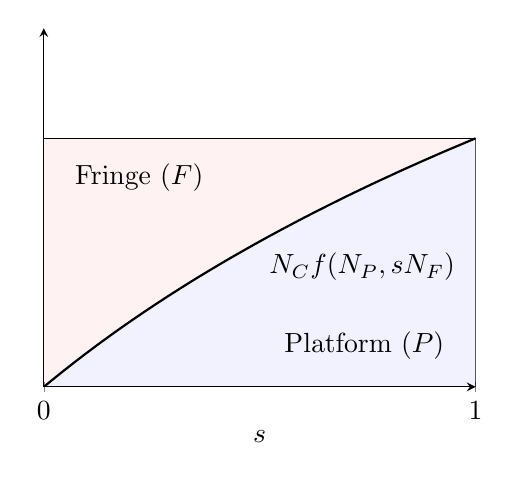
\begin{tikzpicture}[scale=0.8]
            \begin{axis}[xmin=0, xmax=1, ymin=0, ymax=1, samples at={0, 0.02, ..., 0.98, 1},
                xtick={0, 1}, ytick=\empty, axis lines=left, xlabel={$s$}]
                \addplot[name path=f, black, thick] {ln(1+x)};
                % \addplot[name path=tildef, dashed, black] {x};
                \node[anchor=north west] at (axis cs: .5, .4) {$N_C f(N_P, sN_F)$};
                \path[name path=bottom] (axis cs:0,0) -- (axis cs:1,0);
                \draw[name path=top] (axis cs:0,0.693) -- (axis cs:1,0.693);
                \draw[name path=right] (axis cs:1,0) -- (axis cs:1,0.693);
    
                \addplot [fill=blue, fill opacity=0.05] fill between [of=f and bottom];
                \addplot [fill=red, fill opacity=0.05] fill between [of=f and top];
    
                \node[anchor=north west] at (axis cs: .05, .65) {Fringe ($F$)};
                \node[anchor=south east] at (axis cs: .95, .05) {Platform ($P$)};
            \end{axis}
        \end{tikzpicture}
        \caption{Profit shares with $N_P$}
    \end{subfigure}
    \begin{subfigure}[b]{0.45\textwidth}
        \centering
        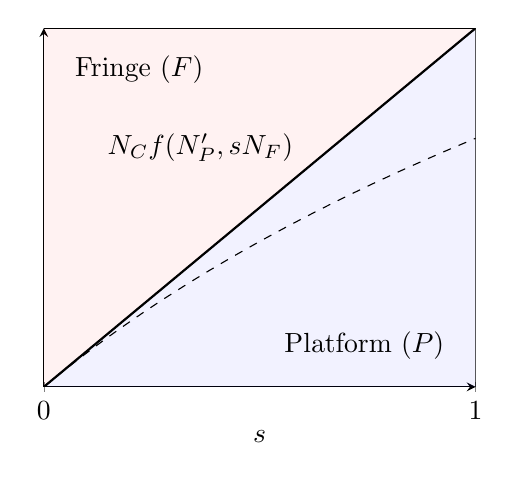
\begin{tikzpicture}[scale=0.8]
            \begin{axis}[xmin=0, xmax=1, ymin=0, ymax=1, samples at={0, 0.02, ..., 0.98, 1},
                xtick={0, 1}, ytick=\empty, axis lines=left, xlabel={$s$}]
                \addplot[name path=f, dashed, black] {ln(1+x)};
                \addplot[name path=tildef, black, thick] {x};
                \node[anchor=south east] at (axis cs: 0.6, 0.6) {$N_C f(N_P', sN_F)$};
                \path[name path=bottom] (axis cs:0,0) -- (axis cs:1,0);
                \draw[name path=top] (axis cs:0,1) -- (axis cs:1,1);
                \draw[name path=right] (axis cs:1,0) -- (axis cs:1,1);
    
                \addplot [fill=blue, fill opacity=0.05] fill between [of=tildef and bottom];
                \addplot [fill=red, fill opacity=0.05] fill between [of=tildef and top];
    
                \node[anchor=north west] at (axis cs: .05, .95) {Fringe ($F$)};
                \node[anchor=south east] at (axis cs: .95, .05) {Platform ($P$)};
            \end{axis}
        \end{tikzpicture}
        \caption{Profit shares with $N_P'$}
    \end{subfigure}
    \caption{Illustration of \cref{prop:share_of_platform} in the one-sided bargaining case. The right hand side figure shows a world with larger platform product variety ($N_P < N_P'$). Even though the platform's share of the total profits is smaller in relative terms in that case, it is still larger in absolute terms.}
    \label{fig:increase_N_P_platform}
\end{figure}

Next, let us look at an analogous result for the fringe firms.
In their case, the direction of the change depends on the complementarities between the fringe firms.
\begin{proposition}
    \label{prop:share_of_fringe}
    Assume that $f, w$ are twice continuously differentiable.
    Let $N_F > 0$.
    Then $\pi_F$ is also differentiable.
    \begin{align*}
        &\text{If } \frac{\partial^2 f(N_P, n_F)}{\partial n_P \partial n_F} < 0 \;\forall n_F \leq N_F, \text{ then } \frac{\partial \pi_F(N_P, N_F)}{\partial N_P} < 0, \\
        &\text{if } \frac{\partial^2 f(N_P, n_F)}{\partial n_P \partial n_F} > 0 \;\forall n_F \leq N_F, \text{ then } \frac{\partial \pi_F(N_P, N_F)}{\partial N_P} > 0
    \end{align*}
    for all $N_P \geq 0$.
\end{proposition}
In summary, when they are mostly substitutes (the cross-derivatives of $f$ are negative), the fringe's profits decrease as a result of an increase in $N_F$.
The intuition is that, even though the total size of the pie increases, the bargaining power of the fringe deteriorates so much that its share decreases not only in relative, but also in absolute terms (as illustrated in \cref{fig:increase_N_P_fringe}).
On the other hand, when the fringe firms are mostly complements the fringe's profits increase.

\begin{figure}[ht]
    \centering
    \begin{subfigure}[b]{0.45\textwidth}
        \centering
        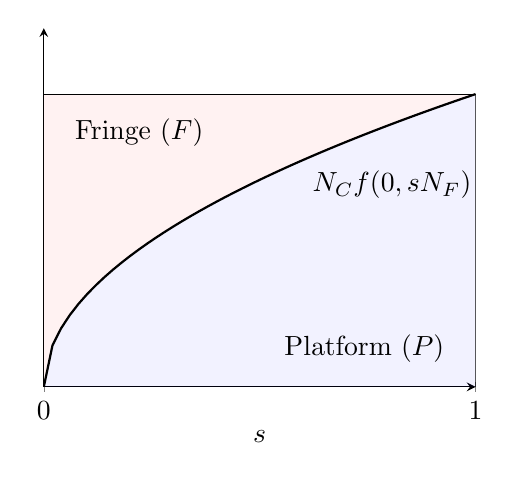
\begin{tikzpicture}[scale=0.8]
            \begin{axis}[xmin=0, xmax=1, ymin=0, ymax=1.225, samples at={0, 0.02, ..., 0.98, 1},
                xtick={0, 1}, ytick=\empty, axis lines=left, xlabel={$s$}]
                \addplot[name path=f, black, thick] {sqrt(x)};
                % \addplot[name path=tildef, dashed, black] {sqrt(0.5+x)};
                \node[anchor=north west] at (axis cs: .6, 0.77) {$N_C f(0, sN_F)$};
                \path[name path=bottom] (axis cs:0,0) -- (axis cs:1,0);
                \draw[name path=top] (axis cs:0,1) -- (axis cs:1,1);
                \draw[name path=right] (axis cs:1,0) -- (axis cs:1,1);
    
                \addplot [fill=blue, fill opacity=0.05] fill between [of=f and bottom];
                \addplot [fill=red, fill opacity=0.05] fill between [of=f and top];
    
                \node[anchor=north west] at (axis cs: .05, .95) {Fringe ($F$)};
                \node[anchor=south east] at (axis cs: .95, .05) {Platform ($P$)};
            \end{axis}
        \end{tikzpicture}
        \caption{Profit shares with $N_P = 0$}
    \end{subfigure}
    \begin{subfigure}[b]{0.45\textwidth}
        \centering
        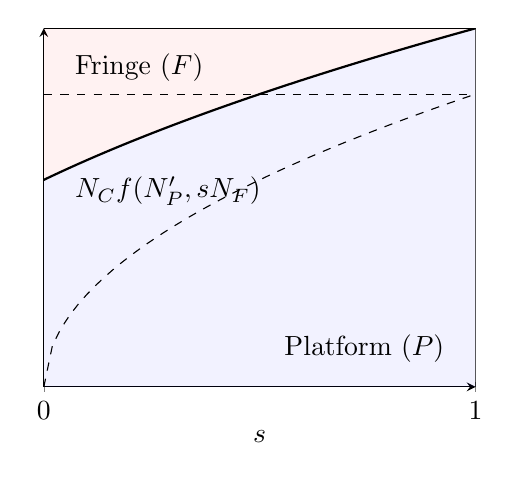
\begin{tikzpicture}[scale=0.8]
            \begin{axis}[xmin=0, xmax=1, ymin=0, ymax=1.225, samples at={0, 0.02, ..., 0.98, 1},
                xtick={0, 1}, ytick=\empty, axis lines=left, xlabel={$s$}]
                \addplot[name path=f, dashed, black] {sqrt(x)};
                \addplot[name path=tildef, black, thick] {sqrt(0.5+x)};
                \node[anchor=north west] at (axis cs: 0.05, 0.75) {$N_C f(N_P', sN_F)$};
                \path[name path=bottom] (axis cs:0,0) -- (axis cs:1,0);
                \draw[name path=top] (axis cs:0,1.225) -- (axis cs:1,1.225);
                \draw[name path=top_old, dashed] (axis cs:0,1) -- (axis cs:1,1);
                \draw[name path=right] (axis cs:1,0) -- (axis cs:1,1.225);
    
                \addplot [fill=blue, fill opacity=0.05] fill between [of=tildef and bottom];
                \addplot [fill=red, fill opacity=0.05] fill between [of=tildef and top];
    
                \node[anchor=north west] at (axis cs: .05, 1.17) {Fringe ($F$)};
                \node[anchor=south east] at (axis cs: .95, .05) {Platform ($P$)};
            \end{axis}
        \end{tikzpicture}
        \caption{Profit shares with $N_P = 0.5$}
    \end{subfigure}
    \caption{Illustration of \cref{prop:share_of_fringe} when fringe and platforrm products are substitutes. An increase in the platform's product variety increases total profits, yet, the fringe's share decreases in absolute terms.}
    \label{fig:increase_N_P_fringe}
\end{figure}

Finally, let us turn to equilibrium entry as a function of the platform's product variety.
The previous proposition implies an almost immediate corollary regarding the equilibrium number of fringe entrants.
\begin{corollary}
    \label{cor:fringe_entry}
    Assume that $f, w$ are twice continuously differentiable.
    Let $N_F^*$ denote the equilibrium number of fringe firms.
    Let us also assume that $N_F^* > 0$, and that
    \begin{align*}
        \frac{\partial^2 f(n_P, n_F)}{\partial n_P \partial n_F} < 0 \quad \forall n_F \leq N_F \\
        \frac{\partial^2 f(n_P, n_F)}{\partial n_F^2} < 0 \quad \forall n_F \leq N_F.
    \end{align*}
    Then the equilibrium number of fringe firms is also differentiable and
    \begin{align*}
        \frac{\partial N_F^*}{\partial N_P} < 0.
    \end{align*}
\end{corollary}
That is, the equilibrium number of entrants increases as a response to an increase in $N_P$ if the fringe firms are mostly complements, and decreases if they are mostly substitutes.
The underlying reason is again the concave or hump-shaped fringe profit function.
If $N_F^*$ is an equilibrium, then fringe profits minus entry costs are strictly positive for all $N_F \leq N_F^*$ and strictly negative for all $N_F > N_F^*$.
Therefore, if an increase in $N_P$ decreases the fringe's profits for every $N_F \geq 0$, equilibrium can be restored by decreasing the number of fringe entrants, (and vice versa for the other case).

Finally, let us conclude this section by establishing a stronger result for a more restrictive class of profit functions.
In the following, I assume that the profit function has an additive form.
Intuitively, this means that -- in terms of total profits generated -- the platform's and the fringe firms' products are substitutable to each other according to some constant ratio.
\begin{assumption}
    \label{ass:additive_profit}
    Assume that $f$ has the following, additive form in $N_P$ and $N_F$:
    \begin{align*}
        f(N_P, N_F) = g(\alpha N_P + \beta N_F)
    \end{align*}
    where $\alpha, \beta > 0$, and $g$ is twice differentiable and that $g'' < 0$.
\end{assumption}

\begin{proposition}
    \label{prop:aggregate_size_additive}
    Let $f$ have the additive form from \cref{ass:additive_profit}.
    Then
    \begin{align*}
        \frac{\partial N_F^*}{\partial N_P} < -\frac{\alpha}{\beta}.
    \end{align*}
    Furthermore,
    \begin{align*}
        \frac{\partial \Pi(N_P, N_F^*(N_P), N_C)}{\partial N_P} < 0.
    \end{align*}
\end{proposition}

The first part of this proposition is a stronger version of \cref{cor:fringe_entry}.
It states that, not only does the equilibrium number of fringe firms decrease as a response to an increase in $N_P$, but it establishes a lower bound for this decrease.
And, as the second part shows, this bound is sufficient to guarantee that the total size of the pie ($\Pi(N_P, N_F, N_C)$) also decreases in equilibrium.

This result has particularly strong implications in models where total profits (or total product variety) has a monotone relationship with consumer welfare, such as those in \textcite{anderson2020aggregative}.
The demand system presented in the main text also has this property.


\section{The platform game and the (weighted) Shapley value}
\label{sec:cooperative_game}

In this section, I describe how the profit sharing rule from \cref{ass:profit_sharing} can be derived from various cooperative games.
In each of the following subsections, I formally define a cooperative game that models the platform setting, and derive the (weighted) Shapley values of the various players.
I show that they correspond to the formulas given in \cref{ass:profit_sharing}, with a specific choice of weight functions $w_P$ and $w_F$ for each case.

I start with the simplest case: one-sided bargaining and the usual Shapley value \parencite{shapley1953additive}.
Then, I look at weighted values \parencite{weber1988probabilistic} in the same cooperative game.
Finally, I consider the case when the consumers also participate in the bargaining process, and derive the corresponding Shapley values.

\subsection{One-sided case}
\label{sec:cooperative_game_one_sided}

In the first setting, the platform and the fringe firms bargain over the total profits they generate together, and the consumers are not included in the negotiations.
The following cooperative game describes this case.

Consider the game $\mathcal{G} = (\mathcal{N}, v)$, characterized by the set of players $\mathcal{N}$ and its characteristic function $v$.
The set of players consists of the platform plus the fringe firms: $\mathcal{N} = \{P, F_i\}, i \in [0, N_F]$.
Because the platform is indispensable, the value of a coalition $S$ is zero without the platform, and depends on the number of fringe firms otherwise:
\begin{align*}
    v(S) = \begin{cases}
        0 & \text{if } P \notin S \\
        N_C f(N_P, n_F(S)) & \text{if } P \in S
    \end{cases},
\end{align*}
where $n_F(S)$ is the measure of fringe firms in $S$.

The following proposition describes the Shapley value of the platform ($\varphi_P(\mathcal{G})$) and the fringe firms ($\varphi_F(\mathcal{G})$) in this game.

\begin{proposition}
    \label{prop:profit_sharing_one_sided}
    Consider the cooperative game above.
    Then, the Shapley values of the platform and the fringe firms are given by
    \begin{align*}
        \varphi_P(\mathcal{G}) &= N_C \int_0^1 f(N_P, s N_F) \ds, \\
        \varphi_P(\mathcal{F}) &= N_C \int_0^1 s N_F \partial_2 f(N_P, s N_F) \ds.
    \end{align*}
\end{proposition}

\begin{proof}[proof of \cref{prop:profit_sharing_one_sided}]
    This result is a direct application of Proposition 3 and Corollary 2 in \textcite{stancsics2023value}.
\end{proof}

As an immediate consequence, if bargaining outcomes are described by the Shapley value, then the resulting allocations satisfy \cref{ass:profit_sharing} with $w_P(s) \equiv 1$ and $w_F(s) = s$.


\subsection{Weighted value}
\label{sec:cooperative_game_weighted}

Now let us generalize the previous result, and assume instead that players' shares are described by their weighted values,
As before, let us start by formally describing the cooperative game.
The set of players and the characteristic function are the same as in \cref{sec:cooperative_game_one_sided}, but now the game is additionally endowed with a weight system $\mathbf{\lambda} = \{\lambda_P, \lambda_{F}(i)\}$.
Let us assume that all fringe players have the same weight $\lambda_{F}(i) \equiv 1$.

Then, the weighted values of the players are described by the following proposition.

\begin{proposition}
    \label{prop:profit_sharing_weighted}
    Consider the cooperative game above.
    Then, the weighted values of the platform and the fringe firms are given by
    \begin{align*}
        \varphi_P(\mathcal{G}) &= N_C \int_0^1 \lambda_P s ^ {\lambda_P - 1} f(N_P, s N_F) \ds, \\
        \varphi_F(\mathcal{G}) &= N_C \int_0^1 s ^ {\lambda_P} N_F \partial_2 f(N_P, s N_F) \ds.
    \end{align*}
\end{proposition}

\begin{proof}[proof of \cref{prop:profit_sharing_weighted}]
    This result is a direct application of Proposition 4 in \textcite{stancsics2023value}.
\end{proof}

As before, the resulting allocations satisfy \cref{ass:profit_sharing} with $w_P(s) \equiv \lambda_P s ^ {\lambda_P - 1}$ and $w_F(s) = s ^ {\lambda_P}$.


\subsection{Two-sided case}
\label{sec:cooperative_game_two_sided}

Finally, in certain settings, it might be appropriate to assume that the consumers (or, more generally, the entities on the other side of the market) also engage in the bargaining process.
The cooperative game describing can be formalized as follows.

The set of players consists of the platform plus the fringe firms: $\mathcal{N} = \{P, F_i, C_j\}, i \in [0, N_F], j \in [0, N_C]$.
The value of a coalition $S$ is zero without the platform, and depends on the number of fringe firms otherwise:
\begin{align*}
    v(S) = \begin{cases}
        0 & \text{if } P \notin S \\
        n_C(S) f(N_P, n_F(S)) & \text{if } P \in S
    \end{cases},
\end{align*}
where $n_F(S)$ and $n_C(S)$ is the measure of fringe firms and consumers, respectively, in $S$.

As in the one-sided case, simple expressions exist for the Shapley value of the platform ($\varphi_P(\mathcal{G})$), fringe firms ($\varphi_F(\mathcal{G})$) and consumers ($\varphi_C(\mathcal{G})$).

\begin{proposition}
    \label{prop:profit_sharing_two_sided}
    Consider the case when only the platform and the fringe firms participate in the bargaining process.
    Then, the resulting profit shares are given by
    \begin{align*}
        \varphi_P(\mathcal{G}) &= N_C \int_0^1 s f(N_P, s N_F) \ds, \\
        \varphi_F(\mathcal{G}) &= N_C \int_0^1 s^2 N_F \partial_2 f(N_P, s N_F) \ds \\
        \varphi_C(\mathcal{G}) &= N_C \int_0^1 s f(N_P, s N_F) \ds.
    \end{align*}
\end{proposition}
\begin{proof}[proof of \cref{prop:profit_sharing_two_sided}]
    This result is a direct application of Proposition 11 in \textcite{stancsics2023value}.
\end{proof}

One thing to note is that the platform's and fringe firms' shares are lower than in the one-sided case.
This is due to the fact of needing to share the pie with the consumers, too.
Additionally, the platform's share is identical to the consumers' (aggregated) share.\footnote{
    This stems from the linearity of the profit function in the number of consumers.
}
This foreshadows the idea that -- even though it might not be welfare-maximizing -- what's good for the platform might also good for the consumers in the two-sided case.
Finally, as in both examples before, these values satisfy \cref{ass:profit_sharing} with $w_P(s) = s$ and $w_F(s) = s^2$.


\section{Non-cooperative microfoundations for the bargaining outcome}
\label{sec:bargaining_microfoundation}

As part of the Nash program\footnote{
    The research agenda aiming to find links between cooperative and non-cooperative game theory, started by nash1953two
}, there have been a number of papers proposing microfoundations for the Shapley value in terms of non-cooperative, bargaining-related games \parencite[e.g.][]{gul1989bargaining,winter1994demand,hart1996bargaining,stole1996intra}.
The cooperative platform game described in \cref{sec:cooperative_game} satisfies the assumption for a number of these models, and thus any of those could be used to build microfoundations for the platform game.
Among those, I will focus on \textcite{stole1996intra} for the reason that it specifically pertains to a setting with one indispensable player and many small players, just like the current paper.

The model in \textcite{stole1996intra} is phrased in terms of intra-firm bargaining between the workers and the firm itself.
The workers are assumed to have a fixed outside option, and the firm is the indispensable player.
This translates directly to the platform game, with the platform being the indispensable player, and fringe firms having a zero outside option.
Furthermore, in \textcite{stole1996intra}, the bargaining outcome is interpreted as the wage for the workers.
In the current setting, this would translate to bargaining over profit shares.
However, as I argue later on, it is equivalent to bargaining over entry fees.
Finally, this section focuses on the main model, with two-sided bargaining, and the Shapley value as the equilibrium concept.
However, the same logic can be applied to the extensions presented in \cref{sec:extensions}, based on sections 3.1 and 3.2 of \textcite{stole1996intra}.

\begin{figure}
    \centering
    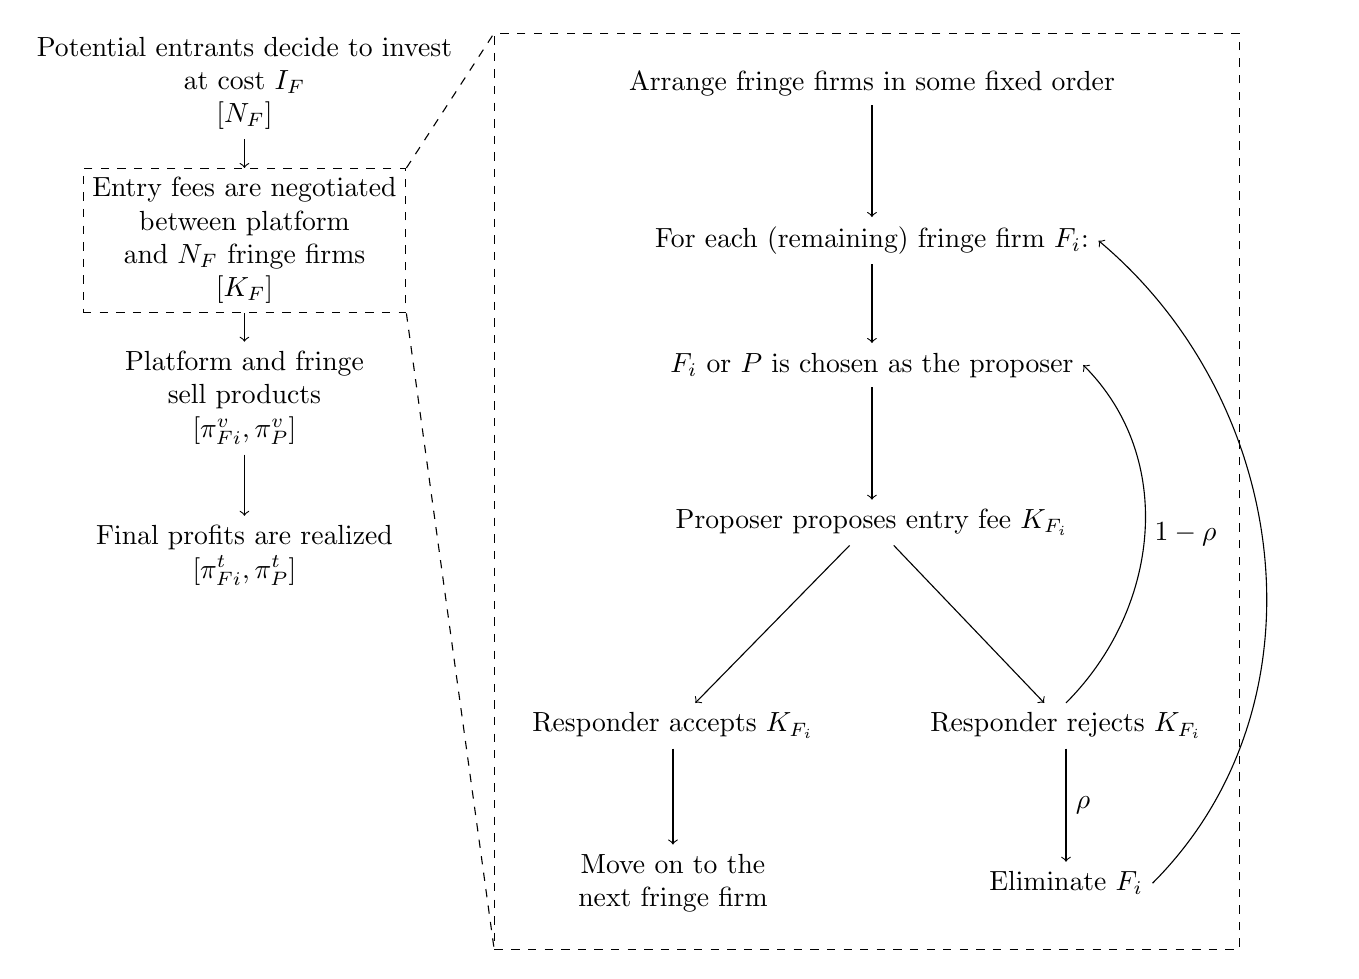
\begin{tikzpicture}[node distance=2cm, auto]
        \node[align=center] (entry_decision) {Potential entrants decide to invest \\ at cost $I_F$ \\ $[N_F]$};
        \node[align=center, draw, dashed] (entry_fee) [below of=entry_decision] {Entry fees are negotiated \\ between platform \\ and $N_F$ fringe firms \\ $[K_F]$};
        \node[align=center] (sales) [below of=entry_fee] {Platform and fringe \\ sell products \\ $[\pi_{Fi}^v, \pi_P^v]$};
        \node[align=center] (final) [below of=sales] {Final profits are realized \\ $[\pi_{Fi}^t, \pi_P^t]$};
        \draw[->] (entry_decision) -- (entry_fee);
        \draw[->] (entry_fee) -- (sales);
        \draw[->] (sales) -- (final);
        
        \node[align=center, right=of entry_decision, distance=3cm] (arrange_fringe) {Arrange fringe firms in some fixed order};
        \node[align=center, below of=arrange_fringe] (foreach) {For each (remaining) fringe firm $F_i$:};
        \node[align=center] (choose_proposer) [below=1cm of foreach] {$F_i$ or $P$ is chosen as the proposer};
        \node[align=center] (proposal) [below of=choose_proposer] {Proposer proposes entry fee $K_{F_i}$};
        \node[align=center] (accept) [below left=2cm and -2cm of proposal] {Responder accepts $K_{F_i}$};
        \node[align=center] (reject) [below right=2cm and -2cm of proposal] {Responder rejects $K_{F_i}$};
        \node[align=center] (next_player) [below of=accept] {Move on to the \\ next fringe firm};
        \node[align=center] (eliminate) [below of=reject] {Eliminate $F_i$};

        \draw[->] (arrange_fringe) -- (foreach);
        \draw[->] (foreach) -- (choose_proposer);
        \draw[->] (choose_proposer) -- (proposal);
        \draw[->] (proposal) -- (accept);
        \draw[->] (proposal) -- (reject);
        \draw[->] (accept) -- (next_player);
        \draw[->] (reject) -- (eliminate) node[midway,right] {$\rho$};

        \draw[->] (reject.north) to [out=45, in=-45] node[midway,right] {$1 - \rho$} (choose_proposer.east);
        \draw[->] (eliminate.east) to [out=45, in=-40] (foreach.east);
        
        \node [draw, dashed, fit=(arrange_fringe)(foreach)(proposal)(accept)(reject)(next_player)(eliminate), inner sep=1em] (expanded_game) {};
        \draw[-, dashed] (entry_fee.north east) -- (expanded_game.north west);
        \draw[-, dashed] (entry_fee.south east) -- (expanded_game.south west);
    \end{tikzpicture}
    \caption{Timing of the model with extensive-form bargaining. The panel on the right-hand side details the negotiation procedure for determining the entry fees.}
    \label{fig:bargaining_microfoundations}
\end{figure}

Let us now describe the bargaining process in the platform game.
First, a random order is determined for the fringe firms.
This order will remain fixed throughout the bargaining phase

Then, for each fringe firm (following the order determined earlier), the platform and the fringe firm negotiate over the entry fee.
This bilateral negotiation follows the alternating offer procedure described in \textcite{binmore1986nash}.
One of the two players is chosen as a proposer, and can propose an entry fee for the given firm: $K_{F_i}$.
The other player can either accept or reject the proposal.

If the proposal is accepted, the negotiation moves on to the next fringe firm.
If it is rejected, with probability $1-\rho$, the other player becomes the proposer, and the negotiation continues.
Finally, with probability $\rho$, the negotiations break down, and the fringe firm is eliminated from the rest of the game.
Crucially, after a breakdown occurs, all of the previous offers are voided, and the platform and the remaining fringe firms start the negotiation process from the beginning (following the same, pre-determined order, but skipping the eliminated firms).

This bargaining process is repeated until all fringe firms have either accepted an offer or been eliminated.
\Cref{fig:bargaining_microfoundations} provides an illustration of the bargaining process, and how it fits into the broader game.
Theorem 2 in \textcite{stole1996intra} shows that regardless of the ordering of the fringe firms, the unique subgame perfect equilibrium of this game is the Shapley value of the cooperative game.
Note, that this result is not only true in expectation: conditioning on any ordering of the fringe firms, the result still holds.

The final piece that is needed to establish the interpretation in terms of entry fees is that for any given configuration of firms emerging from the bargaining process, and, crucially, regardless of the agreed upon entry fees, the unique equilibrium of the subsequent game is the one described in \cref{sec:results_demand}.
According to the previous theorem, players want to agree on a contract such that their final, total profits $\pi^t_{F_i}$ are equal to their Shapley value ($\varphi_{F_i}$).
Given any equilibrium sales profits ($\pi^v_{F_i}$), they can achieve it by setting the entry fees to $K_{F_i} = \varphi_{F_i} - \pi^v_{F_i}$.
Finally, \cref{sec:cooperative_game} and \cref{sec:results_demand} establish that both the Shapley value and the equilibrium sales profits are identical for each fringe firms, and thus a single, common entry fee $K_F$ will be agreed upon.


% \section{The platform's product pricing assumption}
% \label{sec:separate_pricing}

% This section explores the consequences of relaxing the assumption that the platform prices its own products as if they were priced by separate entities.
% So let us now assume, that when pricing product $P_i$, the platform does consider its effect on the sales of its other products.

% For the fringe firms, the problem is the same as before: they choose their prices to maximize their profits, while not having an effect on total aggregate.
% Thus, the price they set is the same as before: $p_{F_i} = c_{F_i} + \mu$.

% The same is not the case with the platform.
% When pricing its products, the platform must consider the effect of its prices on the sales of its other products, through its effects on the aggregate.
% The end result is that the platform will set higher prices than under the separate pricing assumption, because it internalizes the effect of one product's price on the demand for the other products.
% In particular, it can be shown that the optimal price for the platform's product is
% \begin{align*}
%     p_P^* = c_P + \mu + W_0\left( \frac{N_P V_P}{N_F V_F + 1} \right),
% \end{align*}
% where $W_0$ is the principal branch of the Lambert $W$ function.

% Given an aggregate of size $A$, the platform's profits are
% \begin{align*}
%     \dots
% \end{align*}



\section{Proofs and additional lemmas}
\label{sec:proofs}

\begin{lemma}
    \label{lem:single_crossing_affine_transformation}
    Let $g: \mathbb{R}^+ \to \mathbb{R}$ be a twice continuously differentiable function.
    Define
    \begin{align*}
        G(x) = \int_0^1 g(sx) \ds.
    \end{align*}
    Assume that for any $x \geq 0$, $G'(x) < 0$ or $G''(x) < 0$.

    Let $h(x) = c g(a + bx)$ for some $a, c > 0$ and $b > 0$.
    Then the function $H(x) = \int_0^1 h(sx) \ds$ satisfies the same conditions: for any $x \geq 0$, $h'(x) < 0$ or $h''(x) < 0$.
\end{lemma}
\begin{proof}[Proof of \cref{lem:single_crossing_affine_transformation}]
    Differentiating $H$ yields
    \begin{align*}
        H'(x) &= \int_0^1 h'(sx) \ds \\
              &= \int_0^1 c b g'(a + bsx) \ds \\
              &= c b G'(a + bsx).
    \end{align*}
    Similarly, the second derivative is
    \begin{align*}
        H''(x) &= \int_0^1 h''(sx) \ds \\
               &= \int_0^1 c b^2 g''(a + bsx) \ds \\
               &= c b^2 G''(a + bsx).
    \end{align*}
    Now, for any $x \geq 0$, $y = a + bsx \geq 0$, therefore $G'(y) < 0$ or $G''(y) < 0$.
    As $c, b > 0$, this implies that $H'(x) < 0$ or $H''(x) < 0$.
\end{proof}

\begin{lemma}
    \label{lem:slope_at_eq}
    Let the conditions in \cref{ass:single_crossing} hold. Then for any $N_F^* > 0$ for which $\pi_F(N_P, N_F^*, N_C) = I_F(N_F)$, the partial derivative of fringe profits with respect to the number of fringe firms is smaller than the marginal investment cost:
    \begin{align*}
        \left. \frac{\partial \pi_F(N_P, N_F, N_C)}{\partial N_F} \right|_{N_F = N_F^*} < I_F'(N_F).
    \end{align*}
\end{lemma}
\begin{proof}[Proof of \cref{lem:slope_at_eq}]
    \cref{ass:single_crossing} states that at any $N_F \geq 0$, $\pi_F(N_P, N_F, N_C)$ is either concave or decreasing in $N_F$.
    In the remainder, let us denote partial derivatives as follows:
    \begin{align*}
        \partial_F \pi_F(N_P^*, N_F^*, N_C^*) \coloneqq \left. \frac{\partial \pi_F(N_P, N_F, N_C)}{\partial N_F} \right|_{N_P = N_P*, N_F = N_F^*, N_C = N_C^*}.
    \end{align*}

    Notice that the fact that $\pi_F$ is concave or decreasing in $N_F$ implies that if $\partial_F \pi_F(N_P, N_F', N_C)$ for some $N_F' \geq 0$, then $\partial_F \pi_F(N_P, N_F'', N_C) < \partial_F \pi_F(N_P, N_F', N_C)$ for any $\tilde{N_F} < \bar{N_F}$.

    Next, observe that if $\partial_F \pi_F(N_P, 0, N_C) < I_F'(0)$, then there is no equilibrium with $N_F > 0$.
    To show this, assume by contradiction that $\exists N_F^* > 0$ such that $\pi_F(N_P, N_F^*, N_C) = I_F(N_F^*)$.
    Then the mean value theorem implies that there is a $\bar{N}_F \in (0, N_F^*)$ such that $\partial_F \pi_F(N_P, \bar{N}_F, N_C) = I_F'(\bar{N_F}) \geq I_F'(0)$.
    However, this clearly cannot be the case as $\partial_F \pi_F(N_P, N_F, N_C) < I_F'(0)$ or $\pi_F(N_P, N_F, N_C) \leq 0$ for all $N_F > 0$.

    Now let $N_F^*$ be a positive number for which $f(N_P, N_F^*, N_C) = I_F(N_F^*)$.
    It is easy to see that $\partial \pi(N_P, N_F^*, N_C) < I_F'(N_F^*)$.
    The reason is that if it exists, then $\partial_F \pi_F(N_P, 0, N_C) > I_F'(0)$.
    Now if $\partial_F \pi_F(N_P, N_F, N_C) \geq I_F'(N_F) \forall N_F > 0$, then $f(N_P, N_F, N_F) > I_F(N_F)$, and the two functions do not intersect.
    Therefore, there must exist some $\bar{N}_F > 0$ for which $\partial_F \pi_F(N_P, \bar{N}_F, N_C) < I_F'(\bar{N}_F)$.
    This in turn implies that $\partial_F \pi_F(N_P, N_F, N_C) \leq \partial_F \pi_F(N_P, \bar{N}_F, N_C) < I_F'(\bar{N}_F) \leq I_F'(N_F)$ for all $N_F > \bar{N}_F$.
\end{proof}

\begin{proof}[Proof of \cref{prop:unique_equilibrium_more_general}]
    \Cref{lem:slope_at_eq} states that for any positive $N_F^*$ for which $\pi_F(N_P, N_F^*) - N_F I_F$, the partial derivative with respect to the number of fringe firms is negative.
    Now assume by contradiction that $\exists 0 < N_F^* < N_F^{**}$ such that $\pi_F(N_P, N_F^*) = I_F N_F^*$ and $\pi_F(N_P, N_F^{**}) = I_F N_F^{**}$.
    But then the mean value theorem implies that there is a $\bar{N}_F \in (N_F^*, N_F^{**})$ such that $\partial_F \pi_F(N_P, \bar{N}_F) = I_F$.
    This is a contradiction, as $\partial_F \pi_F(N_P, N_F) < I_F$ for all $N_F^* < N_F$.
\end{proof}

\begin{proof}[Proof of \cref{prop:share_of_platform}]
    $f(N_P, N_F)$ is continuously differentiable in $N_P$, therefore the Leibniz rule can be applied to obtain
    \begin{align*}
        \frac{\partial \pi_P(N_P, N_F, N_C)}{\partial N_P} &= N_C \frac{\partial}{\partial N_P} \int_0^1 w_P(s) f(N_P, N_F) \ds \\
        &= \int_0^1 w_P(s) \underbrace{\frac{\partial f(N_P, sN_F)}{\partial N_P}}_{> 0} \ds > 0
    \end{align*}
    for any non-negative, continuous $w_P(s)$.
\end{proof}

\begin{proof}[Proof of \cref{prop:share_of_fringe}]
    Remember that
    \begin{align*}
        \pi_F(N_P, N_F, N_C) = N_C \int_0^1 w_F(s) N_F \partial_2 f(N_P, s N_F) \ds,
    \end{align*}
    By assumption, $f$ is twice continuously differentiable, therefore $\partial_2$ is also continuously differentiable in $N_P$.
    Thus, the Leibniz rule can be applied to obtain
    \begin{align*}
        \frac{\partial \pi_F(N_P, N_F, N_C)}{\partial N_P} &= \frac{\partial}{\partial N_P} N_C \int_0^1 w_F(s) N_F \partial_2 f(N_P, s N_F) \ds \\
        &= N_C \int_0^1 w_F(s) N_F \frac{\partial}{\partial N_P} \partial_2 f(N_P, s N_F) \ds \\
        &= N_C \int_0^1 w_F(s) N_F \partial^2_{12} f(N_P, s N_F) \ds.
    \end{align*}

    As $w_F(s) \geq 0$ for $s > 0$, if $\partial_2 f(N_P, s N_F)$ has the same sign over $[0, N_F]$, then the integral also has the same sign.
    Formally,
    \begin{align*}
        \forall n_F \in [0, N_F] \enspace \frac{\partial^2 f(N_P, n_F)}{\partial N_P \partial n_F} < 0 &\implies \frac{\partial \pi_F(N_P, N_F, N_C)}{\partial N_P} < 0 \\
        \forall n_F \in [0, N_F] \enspace \frac{\partial^2 f(N_P, n_F)}{\partial N_P \partial n_F} > 0 &\implies \frac{\partial \pi_F(N_P, N_F, N_C)}{\partial N_P} > 0
    \end{align*}
\end{proof}

\begin{proof}[Proof of \cref{cor:fringe_entry}]
    \Cref{prop:unique_equilibrium} establishes that if an equilibrium with $N_F > 0$ exists, it is unique.
    Use the implicit function theorem on the equation from \cref{ass:free_entry} to obtain
    \begin{align*}
        \frac{\partial N_F}{\partial N_P} = \frac{\frac{\partial \pi_F(N_P, N_F, N_C)}{\partial N_P}}{I_F'(N_F) - \frac{\partial \pi_F (N_P, N_F, N_C)}{\partial N_F}}
    \end{align*}
    The derivative exists if the above expression is well-defined, i.e. $\frac{\partial \pi_F (N_P, N_F, N_C)}{\partial N_F} \neq I_F$.
    Remember from \cref{prop:share_of_fringe} that the numerator of this expression is negative under the condition $\frac{\partial^2 f(N_P, N_F, N_C)}{\partial N_P \partial N_F}$.
    Now all we need to show to conclude the proof is that
    \begin{align*}
        \frac{\partial \pi_F (N_P, N_F, N_C)}{\partial N_F} < I_F'(N_F),
    \end{align*}
    which is the statement of \cref{lem:slope_at_eq}.
\end{proof}

\begin{proof}[Proof of \cref{prop:aggregate_size_additive}]
    Use the implicit function theorem to get the equilibrium number of fringe firms as a function of the platform's product variety:
    \begin{align*}
        \frac{\partial N_F}{\partial N_P} = \frac{\frac{\partial \pi_F(N_P, N_F, N_C)}{\partial N_P}}{I_F'(N_F) - \frac{\partial \pi_F (N_P, N_F, N_C)}{\partial N_F}}.
    \end{align*}
    Remember, that from \cref{lem:slope_at_eq}, and the assumption on the investment cost function we have that $\frac{\partial \pi_F (N_P, N_F, N_C)}{\partial N_F} < I_F'(N_F)$.
    Then, substitute $f(N_P, N_F) = g(\alpha N_P + \beta N_P)$ into $\pi_F$ to get the following fringe profit function:
    \begin{align*}
        \pi_F(N_P, N_F, N_C) = \beta N_C N_F \int_0^1 w_F(s) g'(\alpha N_P + s \beta N_F) \ds.
    \end{align*}
    Differentiate it with respect to $N_P$ and $N_F$ and substitute into the first expression to obtain
    \begin{align*}
        \frac{\partial N_F}{\partial N_P} = \frac{
            \alpha \beta N_C N_P \int_0^1 w_F(s) g''(\alpha N_P + s \beta N_F) \ds
        }{
            \underbracket{I'_F(N_F) - \beta N_C \int_0^1 w_F(s) g'(\alpha N_P + s \beta N_F) \ds}_{(1)} - \underbracket{\beta^2 N_C N_F \int_0^1 w_F(s) s g''(\alpha N_P + s \beta N_F) \ds}_{(2)}.
        }
    \end{align*}
    From \cref{lem:slope_at_eq}, we know that the denominator of this expression is positive.
    Furthermore, the concavity of $g$ implies that expression (2) is also positive.
    Finally, from \cref{prop:share_of_fringe}, we have that the whole expression must be negative.

    First, let us show that (1) is non-negative, and, coupled with the fact that (2) is positive, omitting it increases the denominator in absolute value, thus making the whole expression larger.
    To see this, observe that the second part of (1) is just the per-unit fringe profit, i.e.
    \begin{align*}
        (1) = I_F'(N_F) - \pi_F(N_P, N_F, N_C) / N_F \geq 0 \Leftrightarrow N_F I_F'(N_F) - \pi_F(N_P, N_F, N_C) \leq 0.
    \end{align*}
    Next, use the convexity of $I_F$ and the definition of the equilibrium to obtain
    \begin{align*}
        N_F I_F'(N_F) - \pi_F(N_P, N_F, N_C) \leq I_F(N_F) - \pi_F(N_P, N_F, N_C) = 0,
    \end{align*}
    thus proving that (1) is non-negative.

    Next, observe that we can bound (2) from above using the fact that $0 \leq s \leq 1$:
    \begin{align*}
        (2) \leq \beta^2 N_C N_F \int_0^1 w_F(s) g''(\alpha N_P + s \beta N_F) \ds.
    \end{align*}
    For the same reason as before, it also bounds the whole expression from above.

    Putting it all together, we have that
    \begin{align*}
        \frac{\partial N_F}{\partial N_P} \leq \frac{\alpha \beta N_C N_P \int_0^1 w_F(s) g''(\alpha N_P + s \beta N_F) \ds}{\beta^2 N_C N_F \int_0^1 w_F(s) g''(\alpha N_P + s \beta N_F) \ds} = -\frac{\alpha}{\beta},
    \end{align*}
    which is the first statement of the proposition.

    To prove the second part of the proposition, differentiate total profits with respect to $N_P$:
    \begin{align*}
        \frac{\partial \Pi(N_P, N_F^*(N_P), N_C)}{\partial N_F} &= \frac{\partial}{\partial N_F} N_C g(\alpha N_P + \beta N_F^*(N_P)) \\
        &= \underbrace{N_C g'(\alpha N_P + \beta N_F^*(N_P))}_{> 0} \left[ \alpha + \beta \frac{\partial N_F^*(N_P)}{\partial N_P} \right] \\
        &< N_C g'(\alpha N_P + \beta N_F^*(N_P)) \left[ \alpha + \beta \left( -\frac{\alpha}{\beta} \right) \right] \\
        &= 0.
    \end{align*}
\end{proof}

\begin{proof}[Proof of \cref{prop:demand_function}]
    See Theorem 1 in \textcite{anderson2021hybrid}.
\end{proof}

\begin{proof}[Proof of \cref{prop:optimal_profit}]
    The profit function for product $Ti$ is the following:
    \begin{align*}
        \pi^v_{T_i}(p_{T_i}) &= (p_{T_i} - c_T) x_{T_i}(p_{Ti}) \\
        &= (p_{T_i} - c_T) \frac{\exp\left( \frac{v_T - p_{T_i}}{\mu} \right)}{A}.
    \end{align*}
    Note that $A$ is not influenced by changes in $p_{T_i}$, as $A$ is an integral and $p_T$ is only changed on a zero-measure (singleton) set.
    Therefore, let calculate the first order condition while treating $A$ as a constant:
    \begin{align}
        \label{eq:foc_profit}
        \mu \frac{\exp\left( \frac{v_T - p_{T_i}}{\mu} \right)}{A} \left[ \frac{p_T - c_T}{\mu} - 1 \right] = 0.
    \end{align}
    Also note that $\pi_{T_i}(p_{T_i})$ is strictly concave, so the FOC is sufficient for optimality.

    Now simply rearrange \cref{eq:foc_profit} to obtain
    \begin{align*}
        p_{T_i}^* = c_T + \mu
    \end{align*}
    and substitute it into the profit function to get
    \begin{align*}
        \pi_{T_i}^{v*} = \mu \frac{\exp \left( \frac{v_T - c_T - \mu}{\mu} \right)}{A}.
    \end{align*}
\end{proof}

\begin{proof}[Proof of \cref{prop:equilibrium_aggregate_benchmark}]
    From \cref{prop:optimal_profit}, the variable profit of each fringe firm is $\pi_{F_i}^{v*} = \mu V_F / A$.
    Total profit after entry fees and investment costs is therefore $\pi_{F_i}^{t*} = \mu V_F / A - I_F - K_F$.
    Under free entry, total profits are zero:
    \begin{align*}
        0 = \pi_{F_i}^{t*} = \mu V_F / A - K_F - I_F.
    \end{align*}
    Simple rearrangement gives the formula we are looking for,
    \begin{align*}
        A = \mu \frac{V_F}{K_F + I_F},
    \end{align*}
    and substituting in $A = N_P V_P + N_F V_F + 1$ yields the equilibrium number of fringe firms,
    \begin{align*}
        N_F = \frac{\mu}{K_F + I_F} - N_P \frac{V_P}{V_F} - \frac{1}{V_F}.
    \end{align*}
\end{proof}

\begin{proof}[Proof of \cref{prop:optimal_entry_fee}]
    The total profit function of the platform is the following:
    \begin{align*}
        \pi_P^t &= \pi_P^v + K_F N_F \\
        &= \mu \frac{N_P V_P}{K_F + I_F} + K_F \left[ \frac{\mu}{K_F + I_F} - N_P \frac{V_P}{V_F} - \frac{1}{V_F} \right].
    \end{align*}
    The function is strictly concave in $K_F$, so the first order condition is sufficient for optimality in the case of an interior solution.
    Assume that that the optimum is indeed interior.
    Then the FOC is
    \begin{align*}
        \frac{\mu I_F V_F - (K_F + I_F)^2}{V_F (K_F + I_F)^2} = 0.
    \end{align*}
    Rearranging it gives the optimal entry fee
    \begin{align*}
        K_F^* = \sqrt{\mu I_F V_F} - I_F,
    \end{align*}
    and substituting it into the profit function leads to
    \begin{align*}
        \pi_P^{*t} = \mu - 2\sqrt{\frac{I_F \mu}{V_F}} + \frac{I_F}{V_F} (N_P V_P + 1).
    \end{align*}
    Finally, note that
    \begin{align*}
        \pi_P^{*t} \geq \mu \frac{N_P V_P}{N_P V_P + 1},
    \end{align*}
    i.e., the profit that the platform could achieve by excluding the fringe completely.
    Therefore, the optimum is indeed interior whenever $K_F$ is low enough

    Now consider the case when $K_F^*$ is so large that it would lead to no fringe entry.
    In that case, the platform's only source of profit is selling its own products, and thus
    \begin{align*}
        \pi_P^{t} = \pi_P^{v} = \mu \frac{ N_P V_P}{N_P V_P + 1}.
    \end{align*}
\end{proof}

\begin{proof}[Proof of \cref{prop:platform_profits_bargaining}]
    Simply integrate the total industry profit function with respect to the mass of fringe entrants obtain the platform's share of the pie:
    \begin{align*}
        \pi^t_P &= \int_0^1 f(N_P, sN_F) \ds \\
        &= \mu \int_0^1 \frac{N_P V_P + s N_F V_F}{N_P V_P + s N_F V_F + 1} \ds \\
        &= \mu \left[ 1 - \frac{\log \left(1 + \frac{N_F V_F}{N_P V_P + 1} \right)}{N_F V_F} \right].
    \end{align*}
    The fringe's share is just the remainder,
    \begin{align*}
        f(N_P, N_F) - \int_0^1 f(N_P, sN_F) \ds = \mu \left[ \frac{\log \left( 1 + \frac{N_F V_F}{N_P V_P + 1} \right)}{N_F V_F} - \frac{1}{N_P V_P + N_F V_F + 1} \right]
    \end{align*}
    Finally, remember that the investment cost of the fringe is fixed at the bargaining stage, and is therefore not included in the bargaining outcome.
    Therefore, the total profits of the complete fringe are
    \begin{align*}
        \pi^t_P = \mu \left[ \frac{\log \left( 1 + \frac{N_F V_F}{N_P V_P + 1} \right)}{N_F V_F} - \frac{1}{N_P V_P + N_F V_F + 1} \right] - I_F N_F.
    \end{align*}
\end{proof}

\begin{proof}[Proof of \cref{lem:shape_of_fringe_profit}]
    First, consider the function
    \begin{align*}
        g(x) = \frac{sx}{1 + sx}.
    \end{align*}
    Also, let us define
    \begin{align*}
        G(x) &= \int_0^1 s g(sx) \ds \\
        &= \frac{\log(x+1)}{x} + \frac{1}{x(x+1)} - \frac{1}{x}.
    \end{align*}

    Differentiation with respect to $x$ yields that
    \begin{align*}
        G'(x) < 0 \iff \log(x+1) > \frac{x (2x+1)}{(x+1)^2}
    \end{align*}
    and
    \begin{align*}
        G''(x) < 0 \iff \log(x+1) < \frac{x (5x^2 + 5x + 2)}{2 (x+1)^3}.
    \end{align*}
    There exists $\bar{x} > 0$\footnote{
        $\bar{x} = 3$ is such a number.
    }, such that the first equality holds for all $x > \bar{x}$, and the second for all $x < \bar{x}$.
    Therefore, $G$ is either concave or decreasing for all $x > 0$.

    Now let us consider the function $h(x) = N_C \mu g(N_P V_P + V_F x)$.
    By \cref{lem:single_crossing_affine_transformation}, $H(x) = \int_0^1 s h'(sx) \ds$ is also either concave or decreasing for any $x > 0$.
    Finally, notice that $H(x)$ is exactly the profit function of the fringe:
    \begin{align*}
        \pi_F(N_P, N_F) = \int_0^1 N_F h'(s N_F) \ds,
    \end{align*}
    thus proving the lemma.
\end{proof}

\begin{proof}[Proof of \cref{prop:unique_equilibrium}]
    \Cref{lem:shape_of_fringe_profit} demonstrates that the fringe total profit function is either concave or decreasing in the number of fringe firms.
    Thus, \cref{ass:single_crossing} is satisfied, and \cref{prop:unique_equilibrium_more_general} implies that the equilibrium number of fringe entrants is unique.
\end{proof}

\begin{proof}[Proof of \cref{prop:fringe_profits_partial}]
    $\pi^t_F(N_P ,N_F)$ adheres to the \cref{ass:identical_fringe,ass:monotone_profits,ass:profit_sharing}.
    Furthermore, 
    \begin{align*}
        \frac{\partial^2 \pi^t_F(N_P ,N_F)}{\partial N_P \partial N_F} < 0 \quad \forall\, N_P, N_F \geq 0.
    \end{align*}
    Therefore, by \cref{prop:share_of_fringe},
    \begin{align*}
        \frac{\partial \pi^t_F(N_P, N_F)}{\partial N_P} < 0 \quad \forall\, N_P, N_F \geq 0.
    \end{align*}
\end{proof}

\begin{proof}[Proof of \cref{prop:N_F_comparative_equilibrium}]
    $\pi^t_F(N_P ,N_F)$ adheres to the \cref{ass:identical_fringe,ass:monotone_profits,ass:profit_sharing,ass:additive_profit}.
    Therefore, by \cref{prop:aggregate_size_additive}
    \begin{align*}
        N_F > 0 \implies \frac{\partial N_F}{\partial N_P} < -\frac{V_P}{V_F}
    \end{align*}
    immediately follows.
\end{proof}

\begin{proof}[Proof of \cref{prop:aggregate_comparative_hybrid}]
    The first statement follows immediately from
    \begin{align*}
        A = N_P V_P + N_F V_F + 1
    \end{align*}
    and
    \begin{align*}
        \frac{\partial N_F}{\partial N_P} < -\frac{V_P}{V_F}
    \end{align*}
    from \cref{prop:N_F_comparative_equilibrium}.
    The second part is a consequence of
    \begin{align*}
        CS \propto \log(A).
    \end{align*}
\end{proof}

\begin{proof}[Proof of \cref{prop:aggregate_comparative_retail}]
    The first statement trivially follows from
    \begin{align*}
        A = N_P V_P + 1.
    \end{align*}
    The second part is a consequence of
    \begin{align*}
        CS \propto \log(A).
    \end{align*}
\end{proof}

\begin{proof}[Proof of \cref{prop:benchmark_results}]
    The respective results are stated in \cref{prop:equilibrium_aggregate_benchmark} and \cref{prop:consumer_surplus_benchmark}.
\end{proof}

\begin{proof}[Proof of \cref{prop:bargaining_results}]
    The respective results are stated in \cref{prop:N_F_comparative_equilibrium} and \cref{prop:aggregate_comparative_hybrid}.
\end{proof}


\end{document}
